\documentclass{beamer}

\usepackage[utf8x]{inputenc} %arregla tema tildes y ñ
\usepackage[activeacute,spanish]{babel}
\usepackage{tikz}
\usepackage{wrapfig} % para meter fotitos volando por ahí
\usepackage[rflt]{floatflt}
\usepackage{graphicx}
\usepackage{subfigure}

\usetikzlibrary{arrows,shapes,arrows,chains,matrix}
%\usepackage[pdftex]{color}

%Tema
\usetheme{Warsaw}
%\usetheme{Berlin}


%\tikzstyle{blockPeque} = [rectangle, draw, thick,draw=gray!80,fill=gray!20,
%text width=80px, text centered, rounded corners, minimum height=13px,node distance = 3cm]

%Portada
\title{RF$^{2}$ - Recarga Fácil por Radio Frecuencia}
\author{Daniel Aicardi, Melina Rabinovich, Edgardo Vaz} 
\institute{
	Tutores: Ing. Juan Pablo Oliver, Ing. Andrés Aguirre\\

\bigskip
\bigskip
	Facultad de Ingeniería - UdelaR\\
	
	\bigskip
	
\includegraphics[scale=.2]{Imagenes/logos.jpg} \\%remove this line if no logo.
}

\date{23 de agosto de 2011}

\begin{document}

%Portada
\begin{frame}[plain]
	\titlepage
\end{frame} 

\begin{frame}
	\frametitle{Temario}
	\begin{itemize}
		\item Introducción
		\item Objetivos
		\item Hardware
		\item Software
		\item Ensayos
		\item Descripción general del funcionamiento
		\item Costos
		\item Posibles Mejoras
		\item Conclusiones y Logros
	\end{itemize}
\end{frame}

\begin{frame}
	\frametitle{Introducción}
	\begin{itemize}
		\item \textcolor{red}{\bf{Introducción}}
		\item \textcolor{gray}{Objetivos}
		\item \textcolor{gray}{Hardware}
		\item \textcolor{gray}{Software}
		\item \textcolor{gray}{Ensayos}
		\item \textcolor{gray}{Descripción general del funcionamiento}		
		\item \textcolor{gray}{Costos}
		\item \textcolor{gray}{Posibles Mejoras}
		\item \textcolor{gray}{Conclusiones y Logros}
	\end{itemize}
\end{frame}

\begin{frame}
	\frametitle{Sistema de transporte}
	\begin {center}
		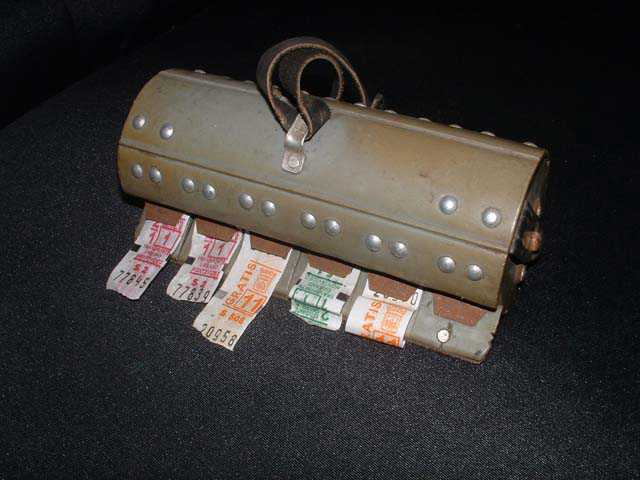
\includegraphics[scale=.3]{Imagenes/boletera.jpg}
		
		\bigskip
		NO más dinero en los ómnibus
	\end{center}
\end{frame}

\begin{frame}
	\frametitle{Sistema de transporte}
	\begin {center}
		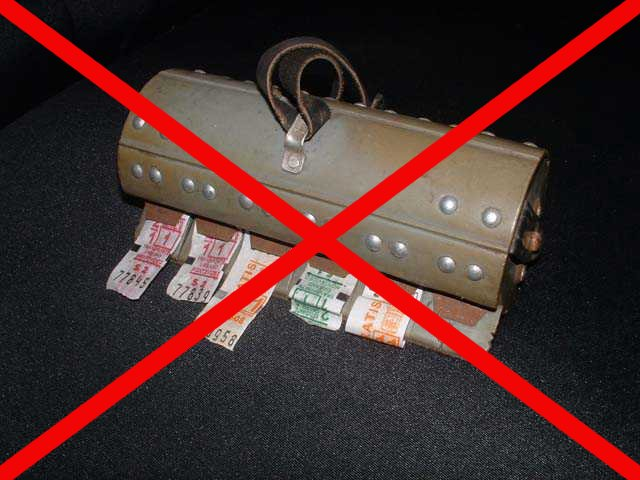
\includegraphics[scale=.3]{Imagenes/boletera_no.jpg}
		
		\bigskip
		NO más dinero en los ómnibus
	\end{center}
\end{frame}


\begin{frame}
	\frametitle{Sistema de transporte}
	\begin{columns}
		\begin{column}{9cm}
			\begin{itemize}
				\item <2-> Tarjeta con saldo para viajar
		
				\bigskip
				\item <3-> Dispositivo lector a bordo que debita viajes

				\bigskip
				\item <4-> Recargar tarjetas
	
				\bigskip
				\item <5-> Modelo de negocio
				\begin{itemize}
					\item <6-> Servidores
					\item <6-> Seguridad
					\item <6-> Puntos de venta
				\end{itemize}
			\end{itemize}
		\end{column}
		
		\begin{column}{3cm}
			\begin{center}	
				\includegraphics <2-> [scale=.15]{Imagenes/tarjeta-STM.png}	
			
				\bigskip	
				\includegraphics <3-> [scale=.1]{Imagenes/labordo.jpg}

				\bigskip
				\includegraphics <5-> [scale=.2]{Imagenes/MrBurns.jpg}
			\end{center}	
		\end{column}
	\end{columns}
\end{frame}

\begin{frame}
	\frametitle{Sistema de transporte - Descripción general}
	\begin{center}	
		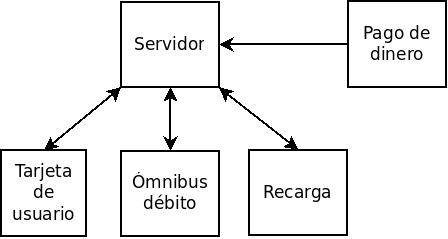
\includegraphics[scale=.5]{Imagenes/sistrans.jpg}
	\end{center}
\end{frame}

\begin{frame}
	\frametitle{Sistema de transporte - Parte a implementar}
	\begin{center}
		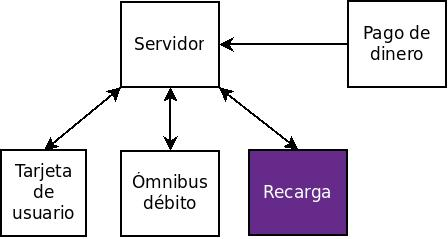
\includegraphics[scale=.5]{Imagenes/sistrans1.jpg}
	\end{center}
\end{frame}

\begin{frame}
	\frametitle{Sistema de transporte - Parte a implementar}
	\begin{center}
		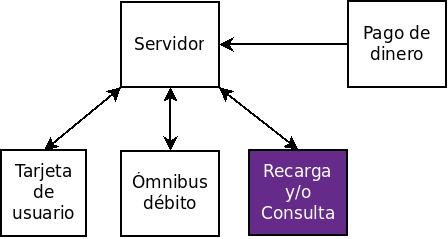
\includegraphics[scale=.5]{Imagenes/sistrans2.jpg}
	\end{center}
\end{frame}	

\begin{frame}
	\frametitle{Sistema de transporte - Funcionamiento actual}	
	\begin{columns}
		\begin{column}{9cm}
			\begin{itemize}
				\item <2-> Mundo PC
		
				\bigskip		
				\item <3-> Puntos de venta concentrados

				\bigskip
				\item <4-> Pago no desacoplado de la recarga

				\bigskip
				\item <5-> No está pensado 24/7		
			\end{itemize}
		\end{column}
		
		\begin{column}{3cm}
			\begin{center}
				\includegraphics <2-> [scale=.05]{Imagenes/pc.jpg}
				
				\bigskip
				\includegraphics <5-> [scale=.2]{Imagenes/no24-7-365.jpg}
			\end{center}
		\end{column}
	\end{columns}
\end{frame}

\begin{frame}
	\frametitle{Sistema de transporte - Funcionamiento alternativo}
	\begin{columns}
		\begin{column}{9cm}
			\begin{itemize}
				\item <2-> Mundo sistemas embebidos

				\bigskip
				\item <3-> Puntos de venta bien distribuidos

				\bigskip
				\item <4-> Pago desacoplado de la recarga

				\bigskip
				\item <5-> 24/7		
			\end{itemize}
		\end{column}
		
		\begin{column}{3cm}
			\begin{center}
				\includegraphics <2-> [scale=.2]{Imagenes/sisemb.jpg}
				
				\bigskip
				\includegraphics <5-> [scale=.2]{Imagenes/24-7-365.jpg}
			\end{center}
		\end{column}
	\end{columns}
\end{frame}

\begin{frame}
	\frametitle{Objetivos}
	\begin{itemize}
		\item \textcolor{gray}{Introducción}
		\item \textcolor{red}{\bf{Objetivos}}
		\item \textcolor{gray}{Hardware}
		\item \textcolor{gray}{Software}
		\item \textcolor{gray}{Ensayos}
		\item \textcolor{gray}{Descripción general del funcionamiento}		
		\item \textcolor{gray}{Costos}
		\item \textcolor{gray}{Posibles Mejoras}
		\item \textcolor{gray}{Conclusiones y Logros}
	\end{itemize}
\end{frame}

\begin{frame}
	\frametitle{Proyecto RF$ ^{2} $ - Objetivos}
		\begin{block} <2-> {Objetivo principal}		
			Diseño y fabricación de un prototipo para recargar y/o consultar tarjetas RFID
		\end{block}

		\bigskip		
		\begin{itemize}			
			\item[] <3-> Características principales del prototipo:

			\bigskip	
			\item <4-> Autónomo

			\bigskip
			\item <4-> Seguro

			\bigskip
			\item <4-> Bajo costo, consumo y mantenimiento
		\end{itemize}

\end{frame}

\begin{frame}
	\frametitle{Hardware}
	\begin{itemize}
		\item \textcolor{gray}{Introducción}
		\item \textcolor{gray}{Objetivos}
		\item \textcolor{red}{\bf{Hardware}}
		\item \textcolor{gray}{Software}
		\item \textcolor{gray}{Ensayos}
		\item \textcolor{gray}{Descripción general del funcionamiento}		
		\item \textcolor{gray}{Costos}
		\item \textcolor{gray}{Posibles Mejoras}
		\item \textcolor{gray}{Conclusiones y Logros}
	\end{itemize}
\end{frame}

\begin{frame}
	\frametitle{Prototipo RF$ ^{2} $ - Sistema de transporte}
	\begin{center}
		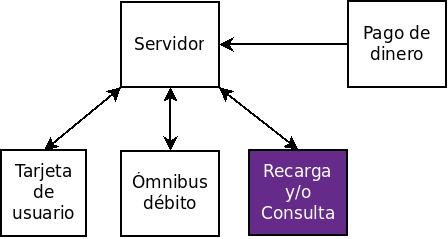
\includegraphics[scale=.5]{Imagenes/sistrans2.jpg}
	\end{center}
\end{frame}	

\begin{frame}
	\frametitle{Prototipo RF$ ^{2} $ - Sistema de transporte}
	\begin{center}
		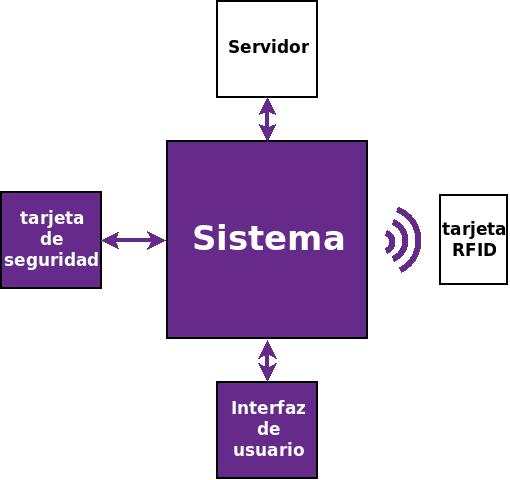
\includegraphics[scale=.35]{Imagenes/diagrama_def.jpg}
	\end{center}
\end{frame}	

\begin{frame}
	\frametitle{Prototipo RF$ ^{2} $ - Descripción}
	\begin{columns}
		\begin{column}{7cm}
			\begin{itemize}
				\item <2-> Sistema basado en un microprocesador (SBC)

				\bigskip
				\item <3-> Lector/escritor de tarjetas RFID %(antena)

				\bigskip
				\item <4-> Lector/escritor de tarjetas de contacto (SAM)

				\bigskip
				\item <5-> Interfaz de usuario
			\end{itemize}
		\end{column}
		\begin{column}{2cm}
			\begin{center}
				\includegraphics <2-> [scale=.06]{Imagenes/sbcgral.jpg}

				\bigskip							
				\includegraphics <3-> [scale=.18]{Imagenes/lectorRF.jpg}

				\bigskip
				\includegraphics <4-> [scale=.1]{Imagenes/sim_card.jpg}			

				\bigskip
				\includegraphics <5-> [scale=.03]{Imagenes/buzzer.jpg}
				\includegraphics <5-> [scale=.03]{Imagenes/leds.jpg}
				\includegraphics <5-> [scale=.06]{Imagenes/displayLCD.jpg}
			\end{center}
		\end{column}
	\end{columns}
\end{frame}

\begin{frame}
	\frametitle{Prototipo RF$ ^{2} $ - Antecedentes}
	\begin{columns}
		\begin{column}{7cm}
			\begin{itemize}
				\item <2-> Existen antecedentes de todas las partes

				\bigskip
				\item <3-> Lectores/escritores de tarjetas RFID y de contacto orientados a PC 

				\bigskip
				\item <4-> OpenPCD - hardware y software abierto

				\bigskip
				\item <5-> AFE - dispositivo autónomo IM
			\end{itemize}	
		\end{column}

		\begin{column}{2.5cm}
			\begin{center}
				\includegraphics <3-> [scale=.2]{Imagenes/le.jpg}
						
				\bigskip
				\includegraphics <4-> [scale=.4]{Imagenes/OpenPCD.jpg}

				\bigskip
				\includegraphics <5-> [scale=.25]{Imagenes/afe.jpg}
			\end{center}
		\end{column}	
	\end{columns}
\end{frame}

\begin{frame}
	\frametitle{Prototipo RF$ ^{2} $ - Elección de arquitecturas}
	\begin{itemize}
		\item <2-> Varias alternativas, muchas similares entre sí

		\bigskip
		\item <3-> Dos más factibles

		\bigskip
		\item[ ] <4-> Arquitectura seleccionada:
	\end{itemize}
	\begin{center}
  		\includegraphics <4-> [scale=.2]{Imagenes/arq.jpg}
	\end{center}
\end{frame}

\begin{frame}
	\frametitle{Arquitectura OpenPCD vs. Prototipo RF$^{2}$}
	\begin{center}
		\scalebox{0.8}{
		\begin{tabular}{c|c}
			OpenPCD & lector/escritor RF$^{2}$ \\ \hline
			dispara los costos & costos razonables\\
			orientado a PC & orientado a sistema embebido\\
			PCB 4 capas & PCB 2 capas\\
			librfid & librfid
		\end{tabular}}	
	\end{center}

	\begin{figure}
		\subfigure{ 
			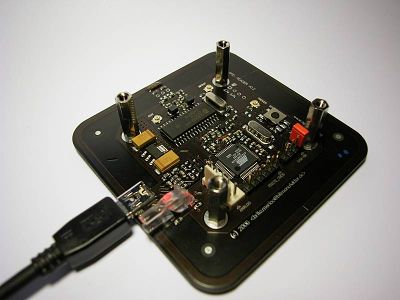
\includegraphics[scale=.9]{Imagenes/OpenPCD.jpg}}
		\subfigure{
  			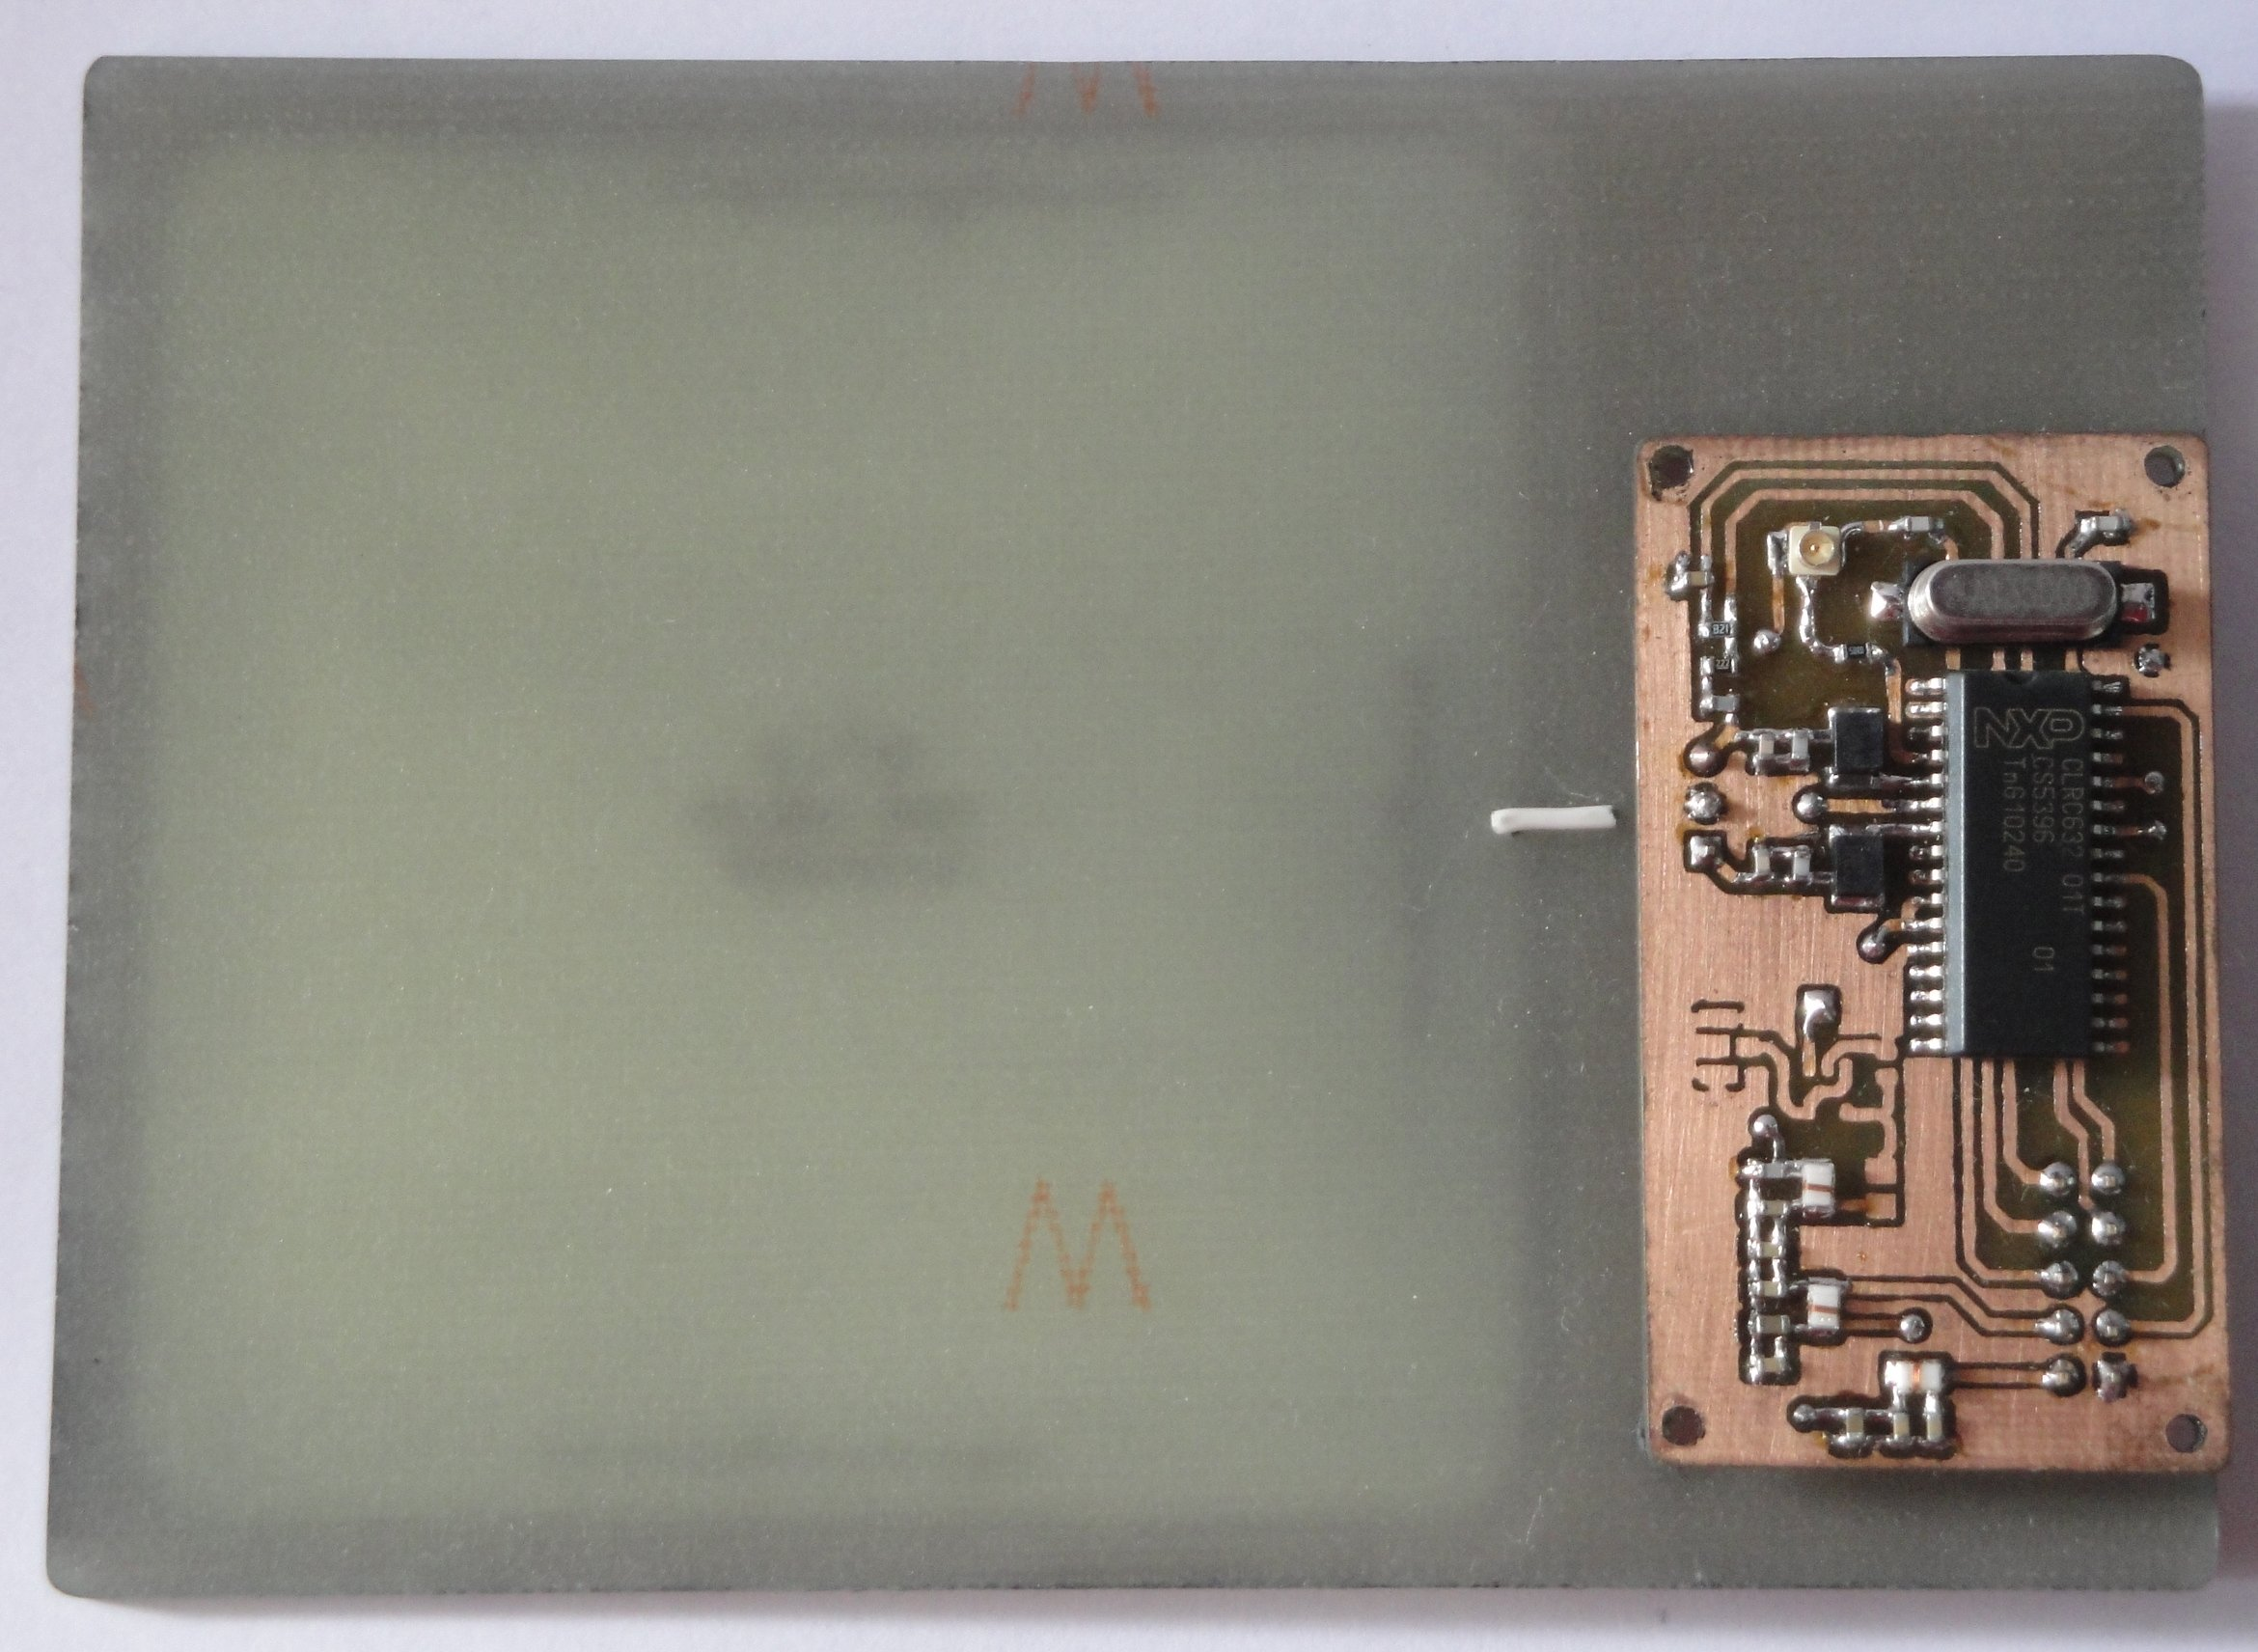
\includegraphics[scale=.04]{Imagenes/ant_b.jpg}} 
	\end{figure}

\end{frame}

\begin{frame}
	\frametitle{Prototipo RF$ ^{2} $}
	\begin{center}
		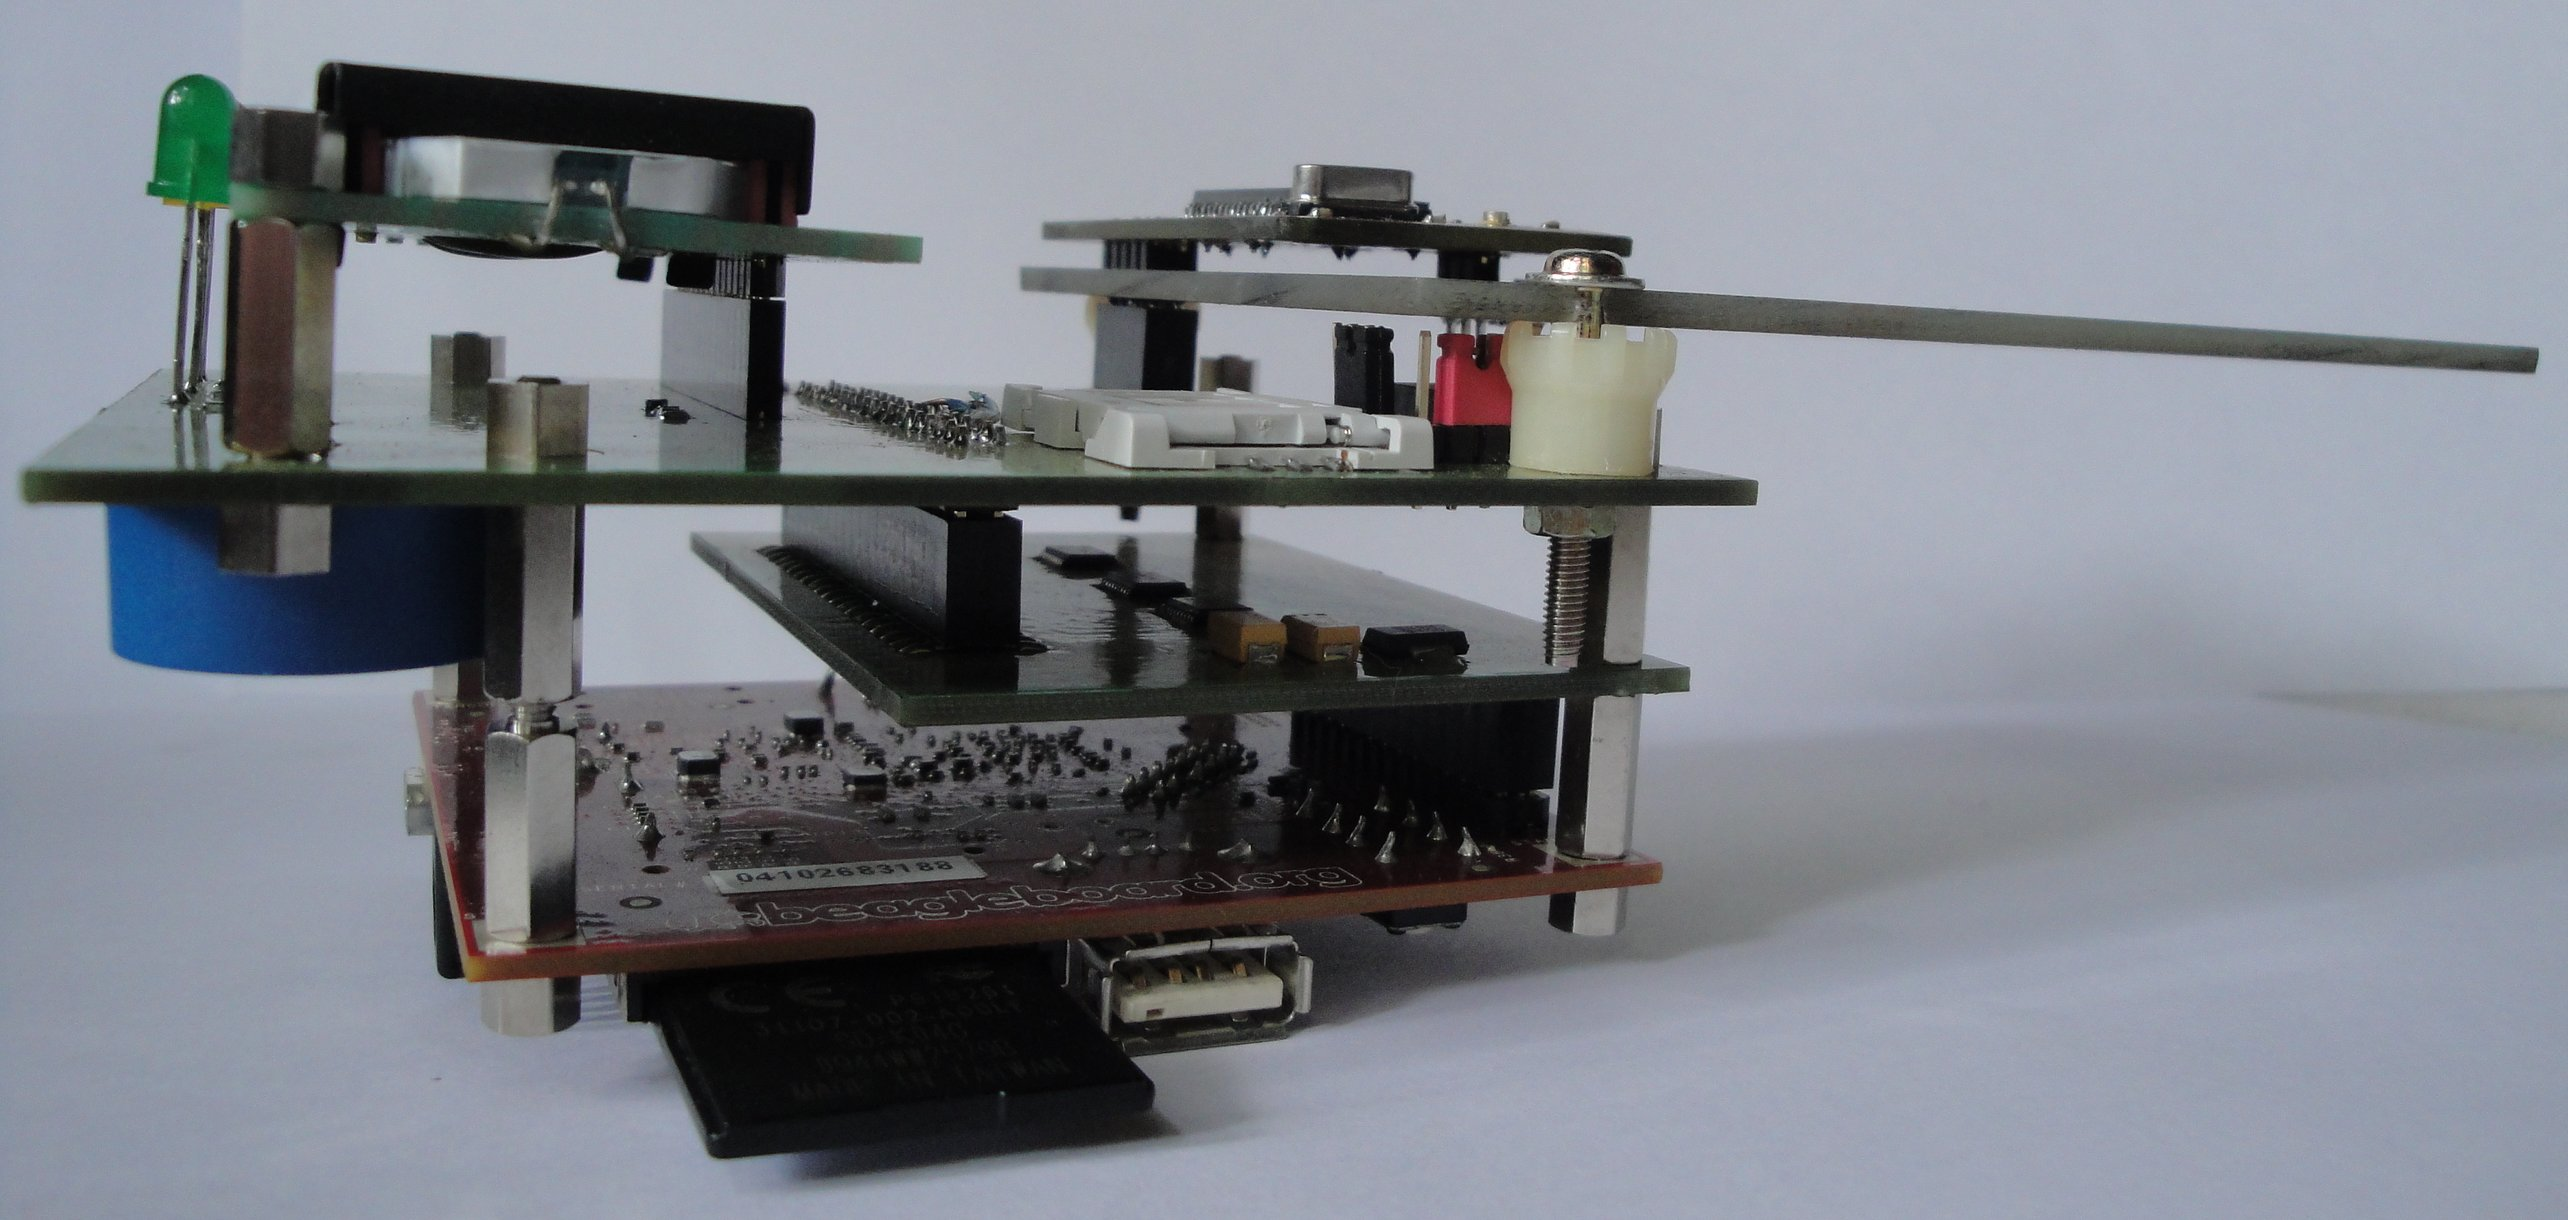
\includegraphics[scale=.12]{Imagenes/prototipo_s.jpg}
	\end{center}
\end{frame}


\begin{frame}
	\frametitle{Prototipo RF$ ^{2} $}
	\begin{center}
		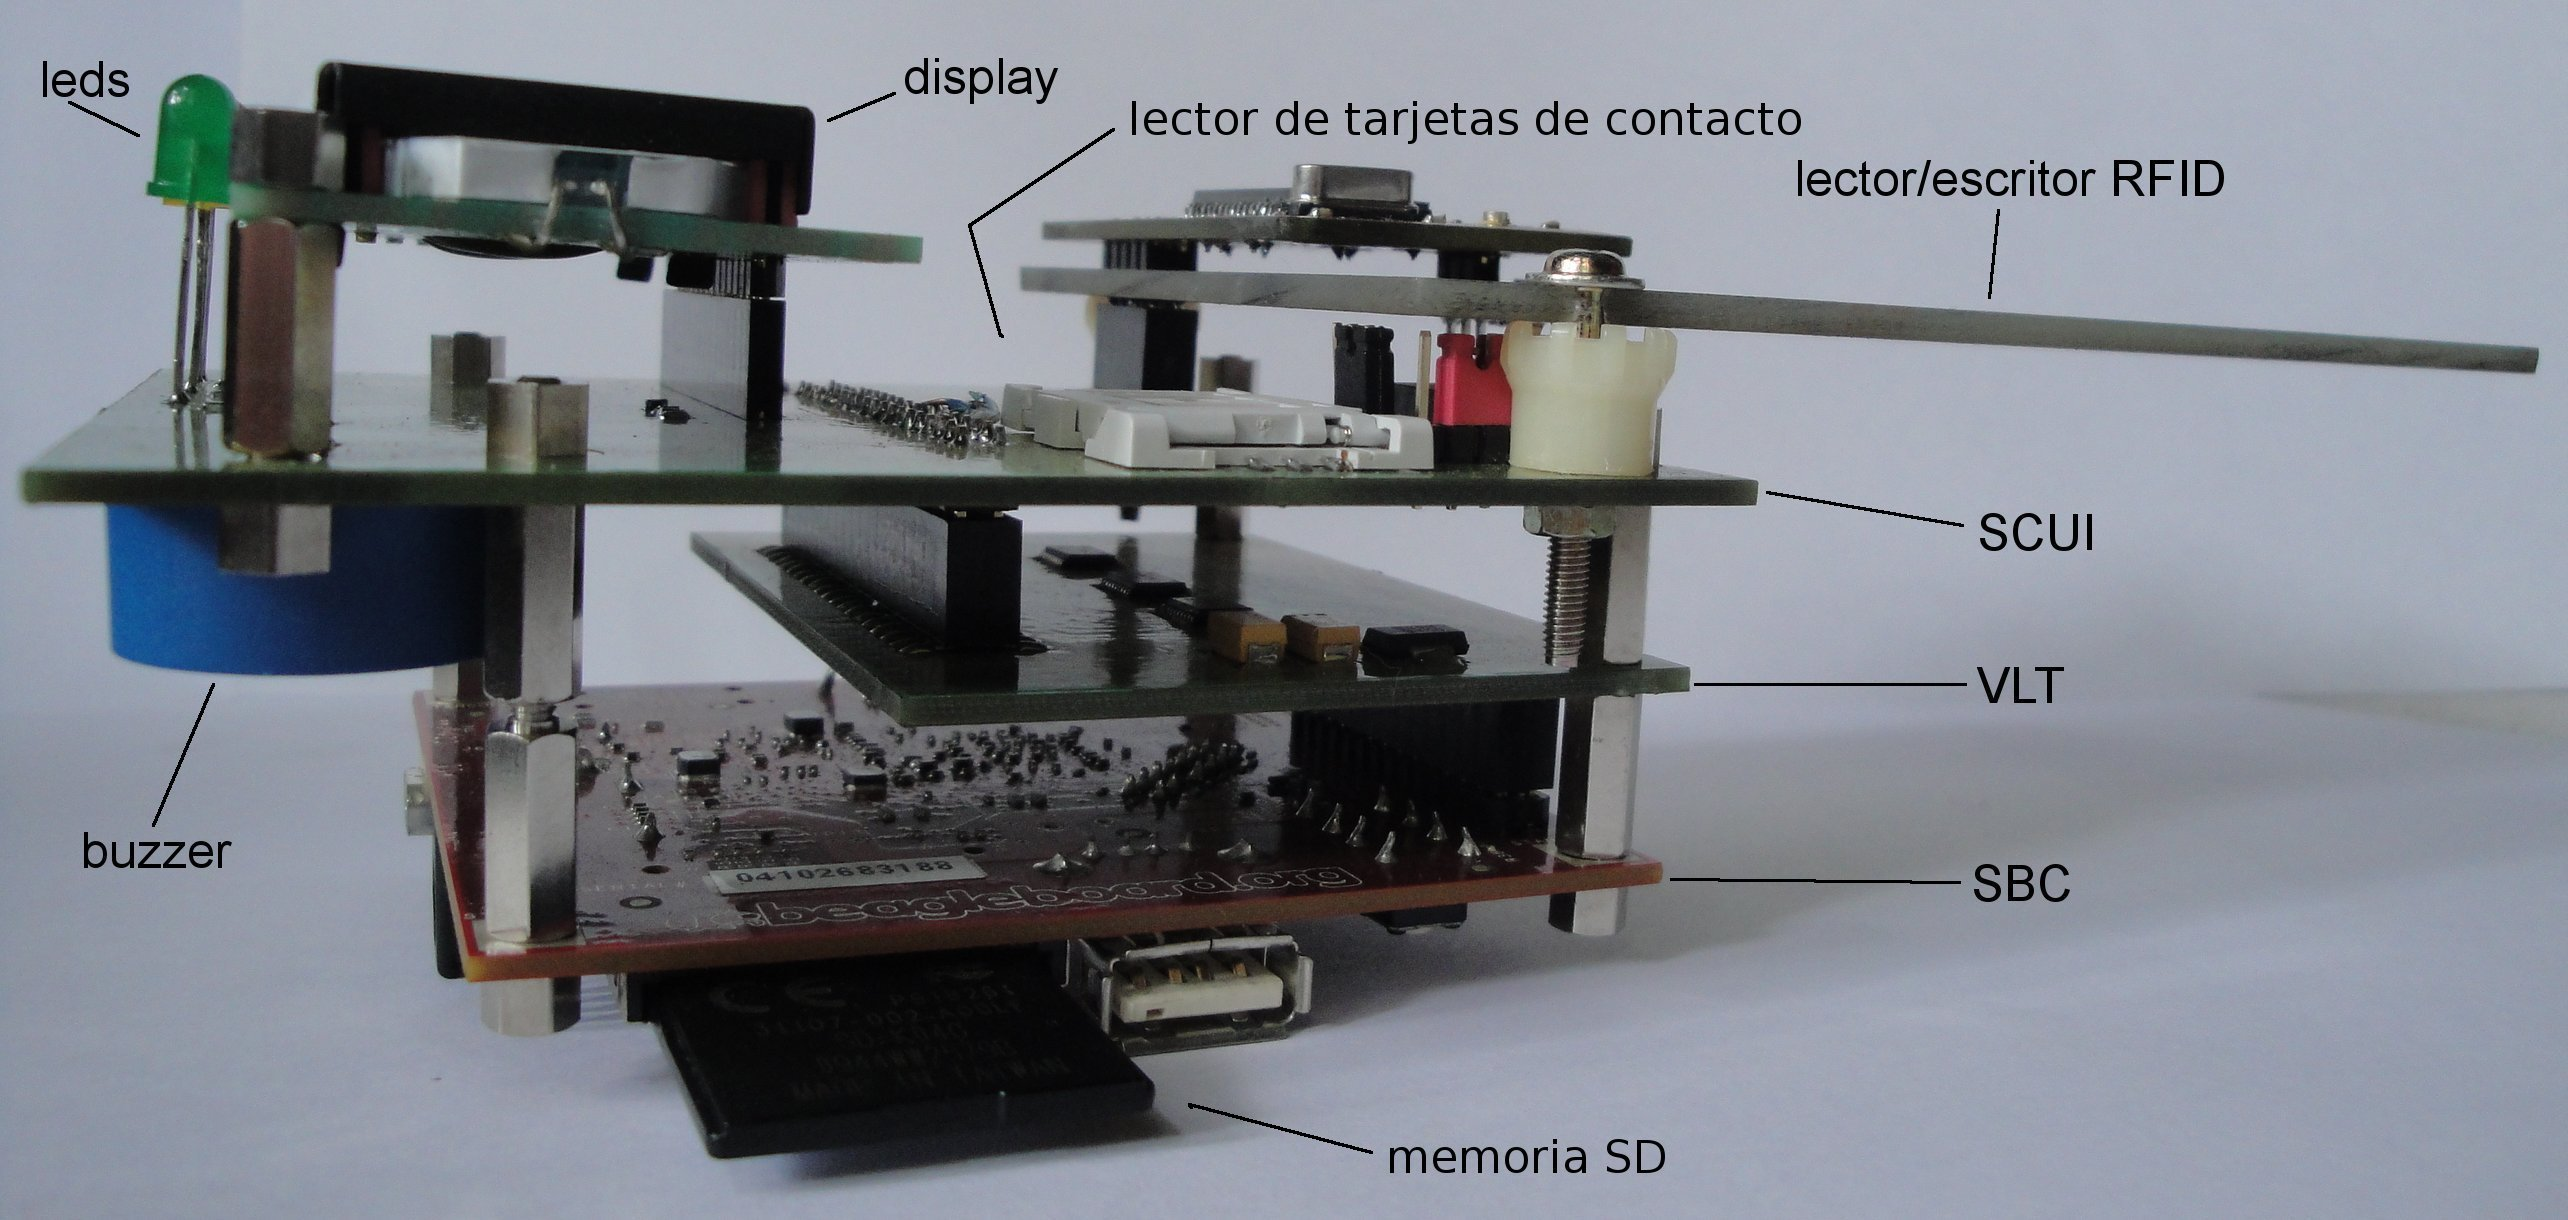
\includegraphics[scale=.12]{Imagenes/prototipo_s_nombres.jpg}
	\end{center}
\end{frame}

\begin{frame}
	\frametitle{Hardware - SBC}
	\begin{itemize}
		\item[] <2-> Beagleboard:
	\end{itemize}
	\begin{figure}
		\centering		
  		\subfigure{
	  		\includegraphics <2-> [scale=.03]{Imagenes/SBC_f.jpg} } 
	  	\subfigure{
	  		\includegraphics <2-> [scale=.03]{Imagenes/SBC_b.jpg} }
	\end{figure}

	\begin{itemize}
		\item <3-> Sistema con microprocesador

		\bigskip
		\item <4-> Adquirido

		\bigskip
		\item <5-> Ejecuta sistema operativo
	\end{itemize}
\end{frame}

\begin{frame}
	\frametitle{Hardware - SCUI}
	\begin{itemize}
		\item[] <2-> Lector de tarjetas de contacto e interfaz de usuario:
	\end{itemize}
	\begin{figure}
		\subfigure{
  			\includegraphics <2->[scale=.03]{Imagenes/SCUI_f.jpg} } 
		\subfigure{ 
			\includegraphics <2-> [scale=.033]{Imagenes/SCUI_b.jpg} }
	\end{figure}

	\begin{itemize}
		\item <3-> Integrados en mismo PCB
		
		\bigskip		
		\item <4-> Lector/escritor de tarjetas de contacto sin ASIC

		\bigskip
		\item <5-> Diseñado y fabricado completamente
	\end{itemize}
\end{frame}

\begin{frame}
	\frametitle{Hardware - lector/escritor RFID}
	\begin{itemize}
		\item[]	<2-> Lector/escritor de tarjetas RFID:
	\end{itemize}
	\begin{figure}
		\subfigure{
  			\includegraphics <2-> [scale=.04]{Imagenes/ant_f.jpg} } 
		\subfigure{ 
			\includegraphics <2-> [scale=.04]{Imagenes/ant_b.jpg} }
	\end{figure}

	\begin{itemize}
		\item <3-> PCB en 2 capas

		\bigskip
		\item <4-> Tarjetas sin contacto (13,56MHz)

		\bigskip
		\item <5-> CL RC632 se encarga del protocolo para las tarjetas (Mifare)

		\bigskip
		\item <6-> Diseñado y fabricado completamente
	\end{itemize}
\end{frame}

\begin{frame}
	\frametitle{Hardware - Tarjetas RFID}
	\begin{columns}
		\begin{column}{8cm}
			\begin{itemize}
				\item <3-> Sin contacto

				\bigskip
				\item <4-> Pasiva

				\bigskip
				\item <5-> Acoplamiento magnético
												
				\bigskip
				\item <6-> Compatibles ISO 14443

				\bigskip
				\item <7-> Mifare 1K - 16 sectores, 4 bloques
				
				\bigskip
				\item <8-> Frecuencia de funcionamiento 13,56MHz

				\bigskip
				\item <9-> CRYPTO1

				\bigskip
				\item <10-> Autenticación por claves, A y B
			\end{itemize}
		\end{column}

		\begin{column}{4cm}
			\begin{center}	
				\includegraphics <2-> [scale=.37]{Imagenes/mifare.jpg}
			\end{center}
		\end{column}
	\end{columns}
	
\end{frame}

\begin{frame}
	\frametitle{Hardware - Tarjetas RFID - Campos de aplicación}
	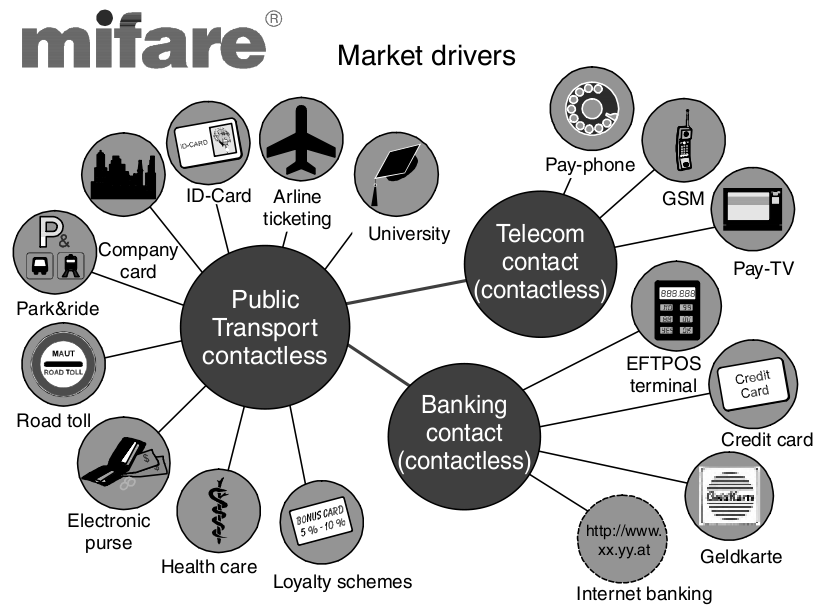
\includegraphics[scale=.35]{Imagenes/aplicaciones.png}
\end{frame}

\begin{frame}
	\frametitle{Software}
	\begin{itemize}
		\item \textcolor{gray}{Introducción}
		\item \textcolor{gray}{Objetivos}
		\item \textcolor{gray}{Hardware}
		\item \textcolor{red}{\bf{Software}}
		\item \textcolor{gray}{Ensayos}
		\item \textcolor{gray}{Descripción general del funcionamiento}		
		\item \textcolor{gray}{Costos}
		\item \textcolor{gray}{Posibles Mejoras}
		\item \textcolor{gray}{Conclusiones y Logros}
	\end{itemize}
\end{frame}

\begin{frame}
	\frametitle{Software}
	\begin{columns}
		\begin{column}{7cm}
			\begin{itemize}
				\item <2-> Sistema Operativo GNU/Linux

				\bigskip
				\item <3-> Distribución Angström

				\bigskip
				\item <4-> Herramientas de desarrollo: 
				\begin{itemize} 
					\item OpenEmbedded-Bitbake 
					\item Narcissus 
				\end{itemize}
			\end{itemize}
		\end{column}
		\begin{column}{4cm}
			\begin{center}
				\includegraphics <2-> [scale=.2]{Imagenes/linux.jpg}
				
				\bigskip
				\includegraphics <3-> [scale=.3]{Imagenes/Angstrom.png}				
			\end{center}
		\end{column}
	\end{columns}
\end{frame}		

\begin{frame}
	\frametitle{Software - Sistema Operativo}
	\begin{center}
		\includegraphics <2-> [scale=.3]{Imagenes/sd.jpg}
	\end{center}
	\begin{itemize}		
		\item[] <3-> Estructura de memoria SD
	\end{itemize}
	\begin{itemize}
		\item <4-> fileSystem, sistema de archivos de la distribución seleccionada

		\bigskip
		\item <5-> uImage, es el kernel comprimido del sistema

		\bigskip
		\item <6-> uboot.bin y MLO, forman parte del bootloader
	\end{itemize}
\end{frame}

\begin{frame}
	\frametitle{Software - Bibliotecas}
	\begin{itemize}
		\item <2-> librfid, editada (utilizada por librfid-tool)

		\bigskip
		\item <3-> libgpio, completamente implementada

		\bigskip
		\item <4-> liblcd, editada (implementada para Audio Fingerprint)

		\bigskip
		\item <5-> libpcsclite
	\end{itemize}
	\begin{center}
		\includegraphics <6-> [scale=.3]{Imagenes/SW.jpg}
	\end{center}
\end{frame}

\begin{frame}
	\frametitle{Software - librfid-tool}
	\begin{center}
		\includegraphics <2-> [scale=.3]{Imagenes/librfid-tool.jpg}
	\end{center}
	\begin{itemize}		
		\item[] <3-> Funciones de utilidad de la herramienta librfid-tool:
	\end{itemize}
	\begin{itemize}
		\item <4-> Lectura de tarjeta completa

		\bigskip
		\item <5-> Lectura de un bloque específico

		\bigskip
		\item <6-> Escritura de un bloque específico
	\end{itemize}
\end{frame}

\begin{frame}
	\frametitle{Diagrama de flujo}
	\begin{center}
		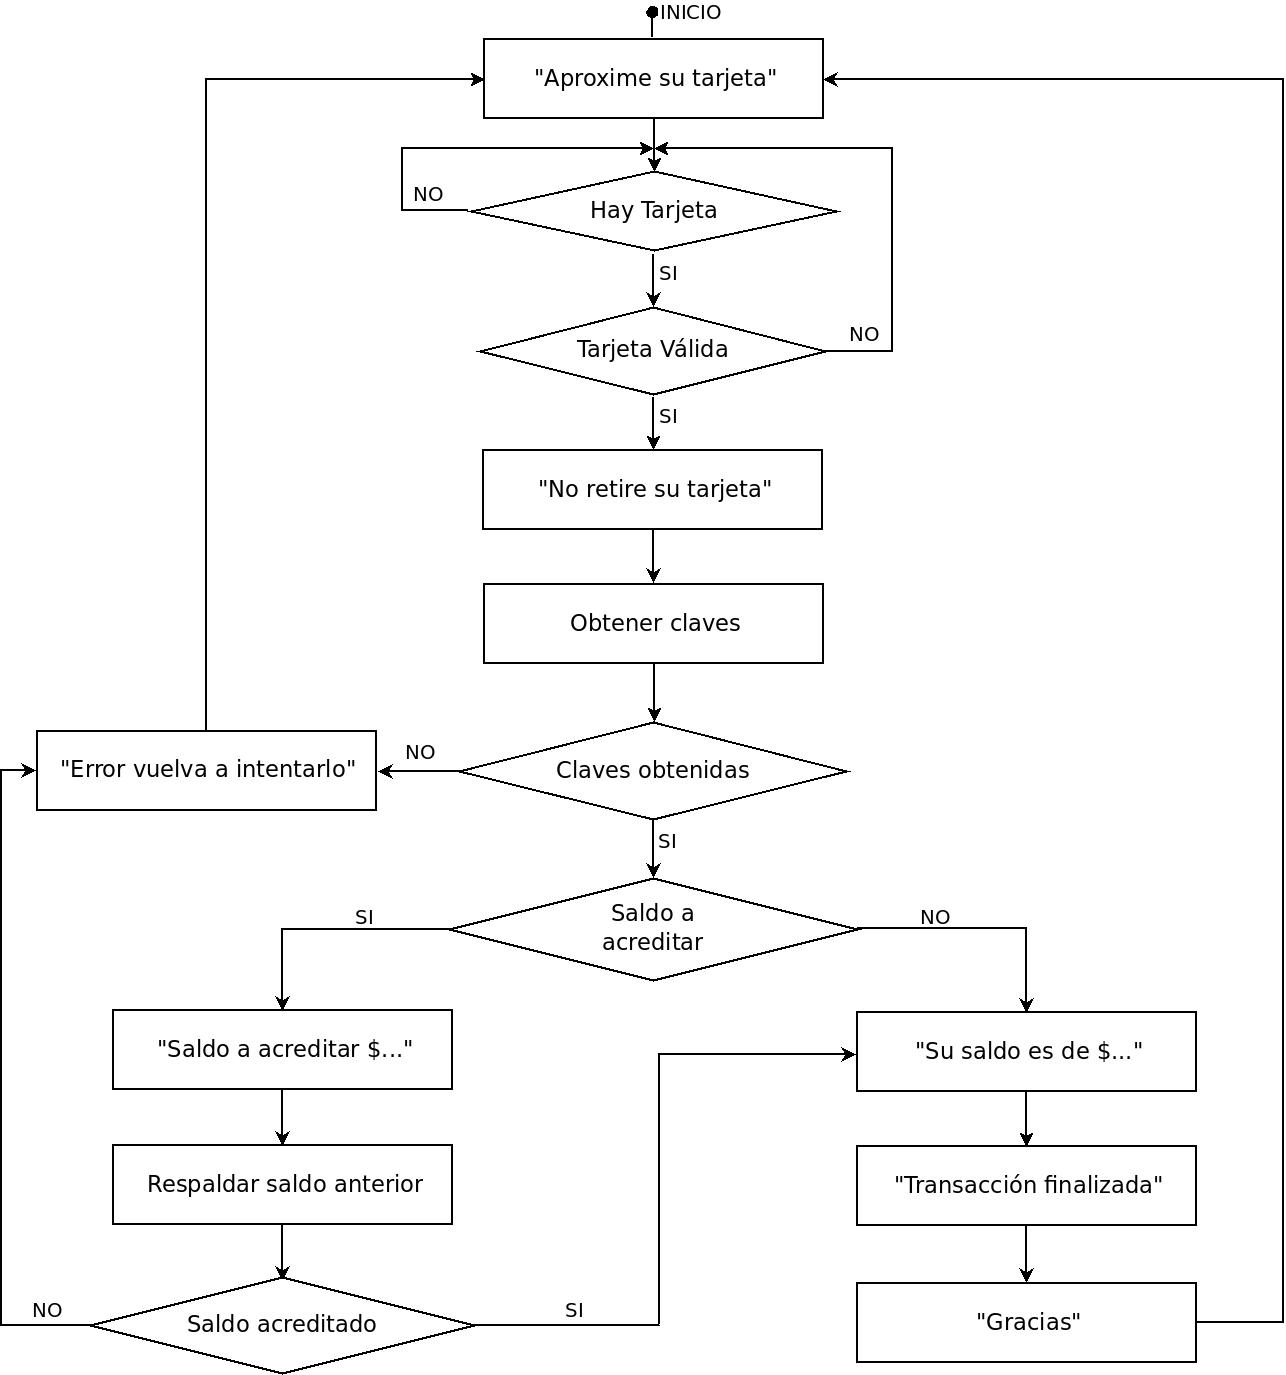
\includegraphics[scale=.166]{Imagenes/flujo.jpg}
	\end{center}
\end{frame}	

\begin{frame}
	\frametitle{Ensayos}
	\begin{itemize}
		\item \textcolor{gray}{Introducción}
		\item \textcolor{gray}{Objetivos}
		\item \textcolor{gray}{Hardware}
		\item \textcolor{gray}{Software}
		\item \textcolor{red}{\bf{Ensayos}}
		\item \textcolor{gray}{Descripción general del funcionamiento}		
		\item \textcolor{gray}{Costos}
		\item \textcolor{gray}{Posibles Mejoras}
		\item \textcolor{gray}{Conclusiones y Logros}
	\end{itemize}
\end{frame}

\begin{frame}
	\frametitle{Ensayos - SBC}
	\begin{columns}
		\begin{column}{9cm}	
			\begin{itemize}
				\item <2-> Hawkboard	
				\begin{itemize}
					\item <3-> Errores en el booteo
					\item <3-> Se bloquea
					\item[ ] <4-> Solución: \underline{cambio de SBC}
				\end{itemize}

				\bigskip			
				\item <5-> Beagleboard
				\begin{itemize}
					\item <6-> Incompatibilidad de niveles de tensión
					\item[ ] <7-> Solución: \underline{VLT}

					\bigskip
					\item <8-> Atributos de GPIOs por u-boot, no fue posible
					\item[ ] <9-> Solución: \underline{hacerlo por kernel}
					
					\bigskip					
					\item <10-> Problemas con memoria SD
					\item[ ] <11-> Solución: \underline{sustituirla, tenía bloques rotos}
				\end{itemize}
			\end{itemize}
		\end{column}	
		\begin{column}{3.5cm}		
			\begin{center}
				\includegraphics <3-> [scale=.3]{Imagenes/preg.jpg}
			\end{center}
		\end{column}
	\end{columns}
\end{frame}

\begin{frame}
	\frametitle{Ensayos - SCUI}
	\begin{itemize}
		\item <2-> UI - Interfaz de usuario
		\begin{itemize}		
			\item <3-> Errores de impresión en el display
			\item[ ] <4-> Solución: \underline{cambio de caracteres ASCII}
	\end{itemize}

	\bigskip
	\item <5-> SC - Lector/escritor de tarjetas de contacto
		\begin{itemize}
			\item <6-> Oscilador de frecuencia inadecuada
			\item[ ] <7-> Solución: \underline{cambio de oscilador - 3,579545MHz}

			\bigskip
			\item <8-> PCB VLT causó problemas en la recepción
			\item[ ] <9-> Solución: \underline{cambiar resistencia en el lector/escritor}
		\end{itemize}	
	\end{itemize}
\end{frame}

\begin{frame}
	\frametitle{Ensayos - lector/escritor RFID}
	\begin{columns}
		\begin{column}{9cm}
			\begin{itemize}
				\item <2-> Testeo hardware en un rabbit por falta de SBC
		
				\bigskip
				\item <3-> La antena no genera campo magnético
				\item[ ] <5-> Solución: \underline{bobina externa al PCB}

				\bigskip		
				\item <6-> Error en el circuito de matcheo 
				\item[ ] <7-> Solución: \underline{cambio de capacitores}
		
				\bigskip
				\item <8-> Problemas al leer tarjetas
				\item[ ] <9-> Solución: \underline{cambio de f$_{clk}$ del puerto de}
										\underline{comunicación}

		
				\bigskip
				\item <10-> Varias modificaciones en herramienta librfid-tool
			\end{itemize}
		\end{column}
		
		\begin{column}{4cm}
			\begin{center}
				\includegraphics <4-> [scale=.6]{Imagenes/no.jpg}

				\bigskip
				\includegraphics <5-> [scale=.025]{Imagenes/ant_rulo.jpg}
			\end{center}
		\end{column}
	\end{columns}
\end{frame}


\begin{frame}
	\frametitle{Costos}
	\begin{itemize}
		\item \textcolor{gray}{Introducción}
		\item \textcolor{gray}{Objetivos}
		\item \textcolor{gray}{Hardware}
		\item \textcolor{gray}{Software}
		\item \textcolor{gray}{Ensayos}
		\item \textcolor{red}{\bf{Descripción general del funcionamiento}}
		\item \textcolor{gray}{Costos}
		\item \textcolor{gray}{Posibles Mejoras}
		\item \textcolor{gray}{Conclusiones y Logros}
	\end{itemize}
\end{frame}


%%%%%%%%%%%%%%%%%

\begin{frame}
	\frametitle{Descripción general de funcionamiento}
	\begin{center}
		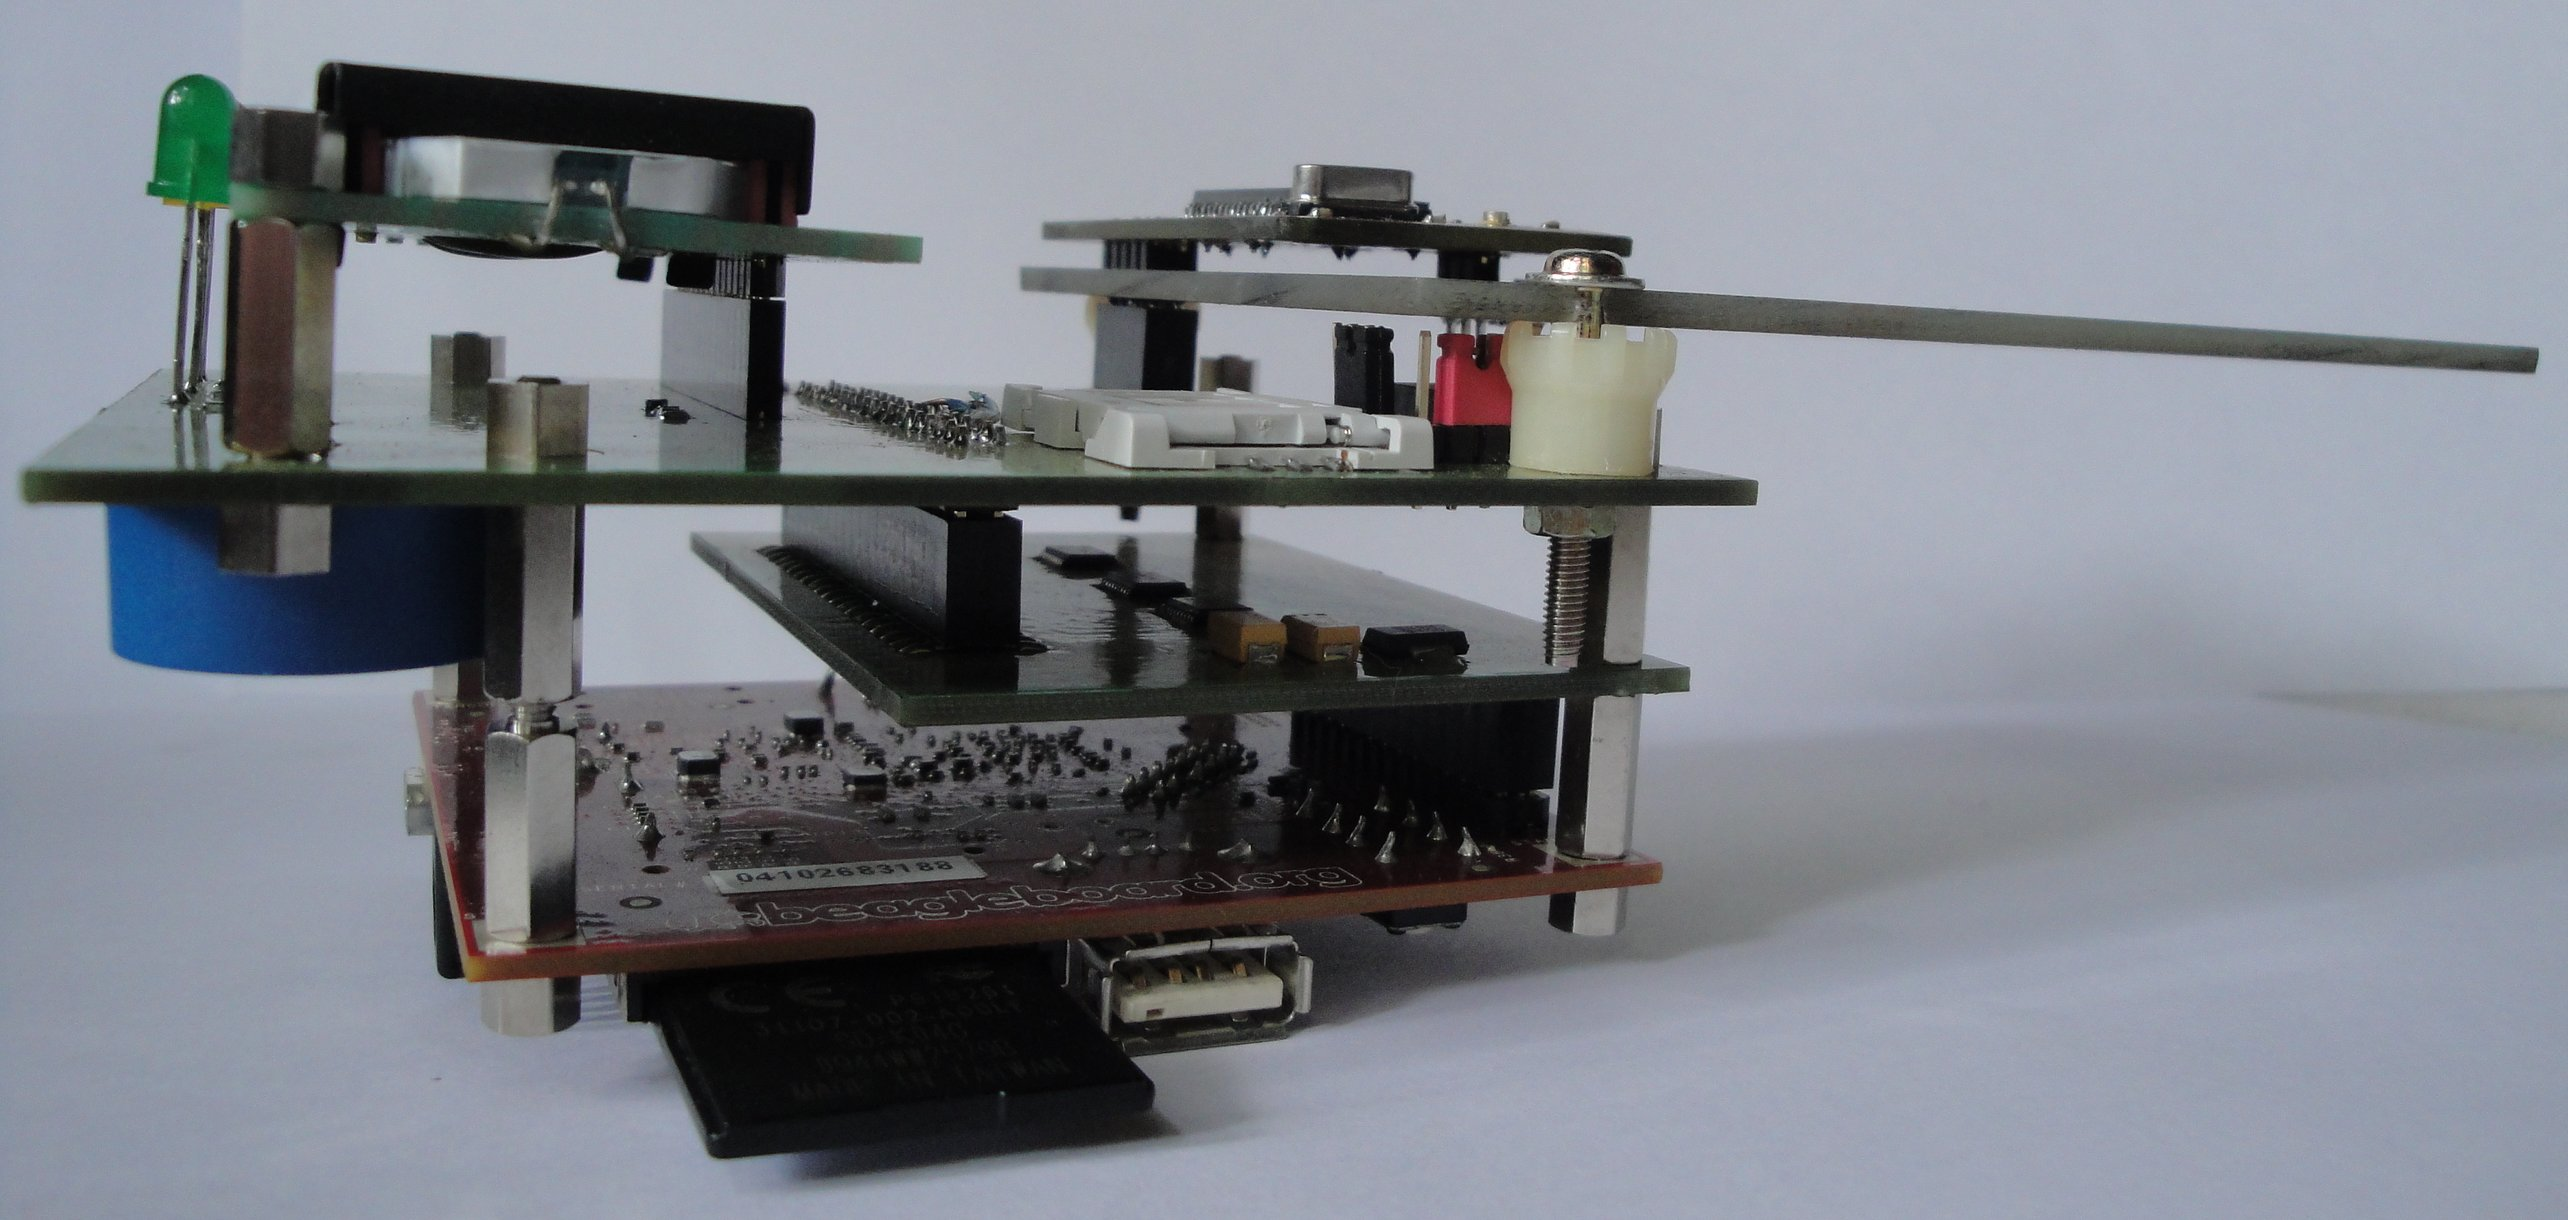
\includegraphics[scale=.08]{Imagenes/prototipo_s.jpg}
		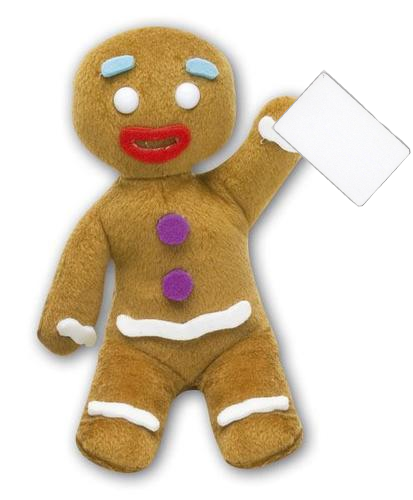
\includegraphics[scale=.35]{Imagenes/pinpon_tarj.png}
	\end{center}
\end{frame}	

\begin{frame}
	\frametitle{Descripción general de funcionamiento}
	\begin{center}
		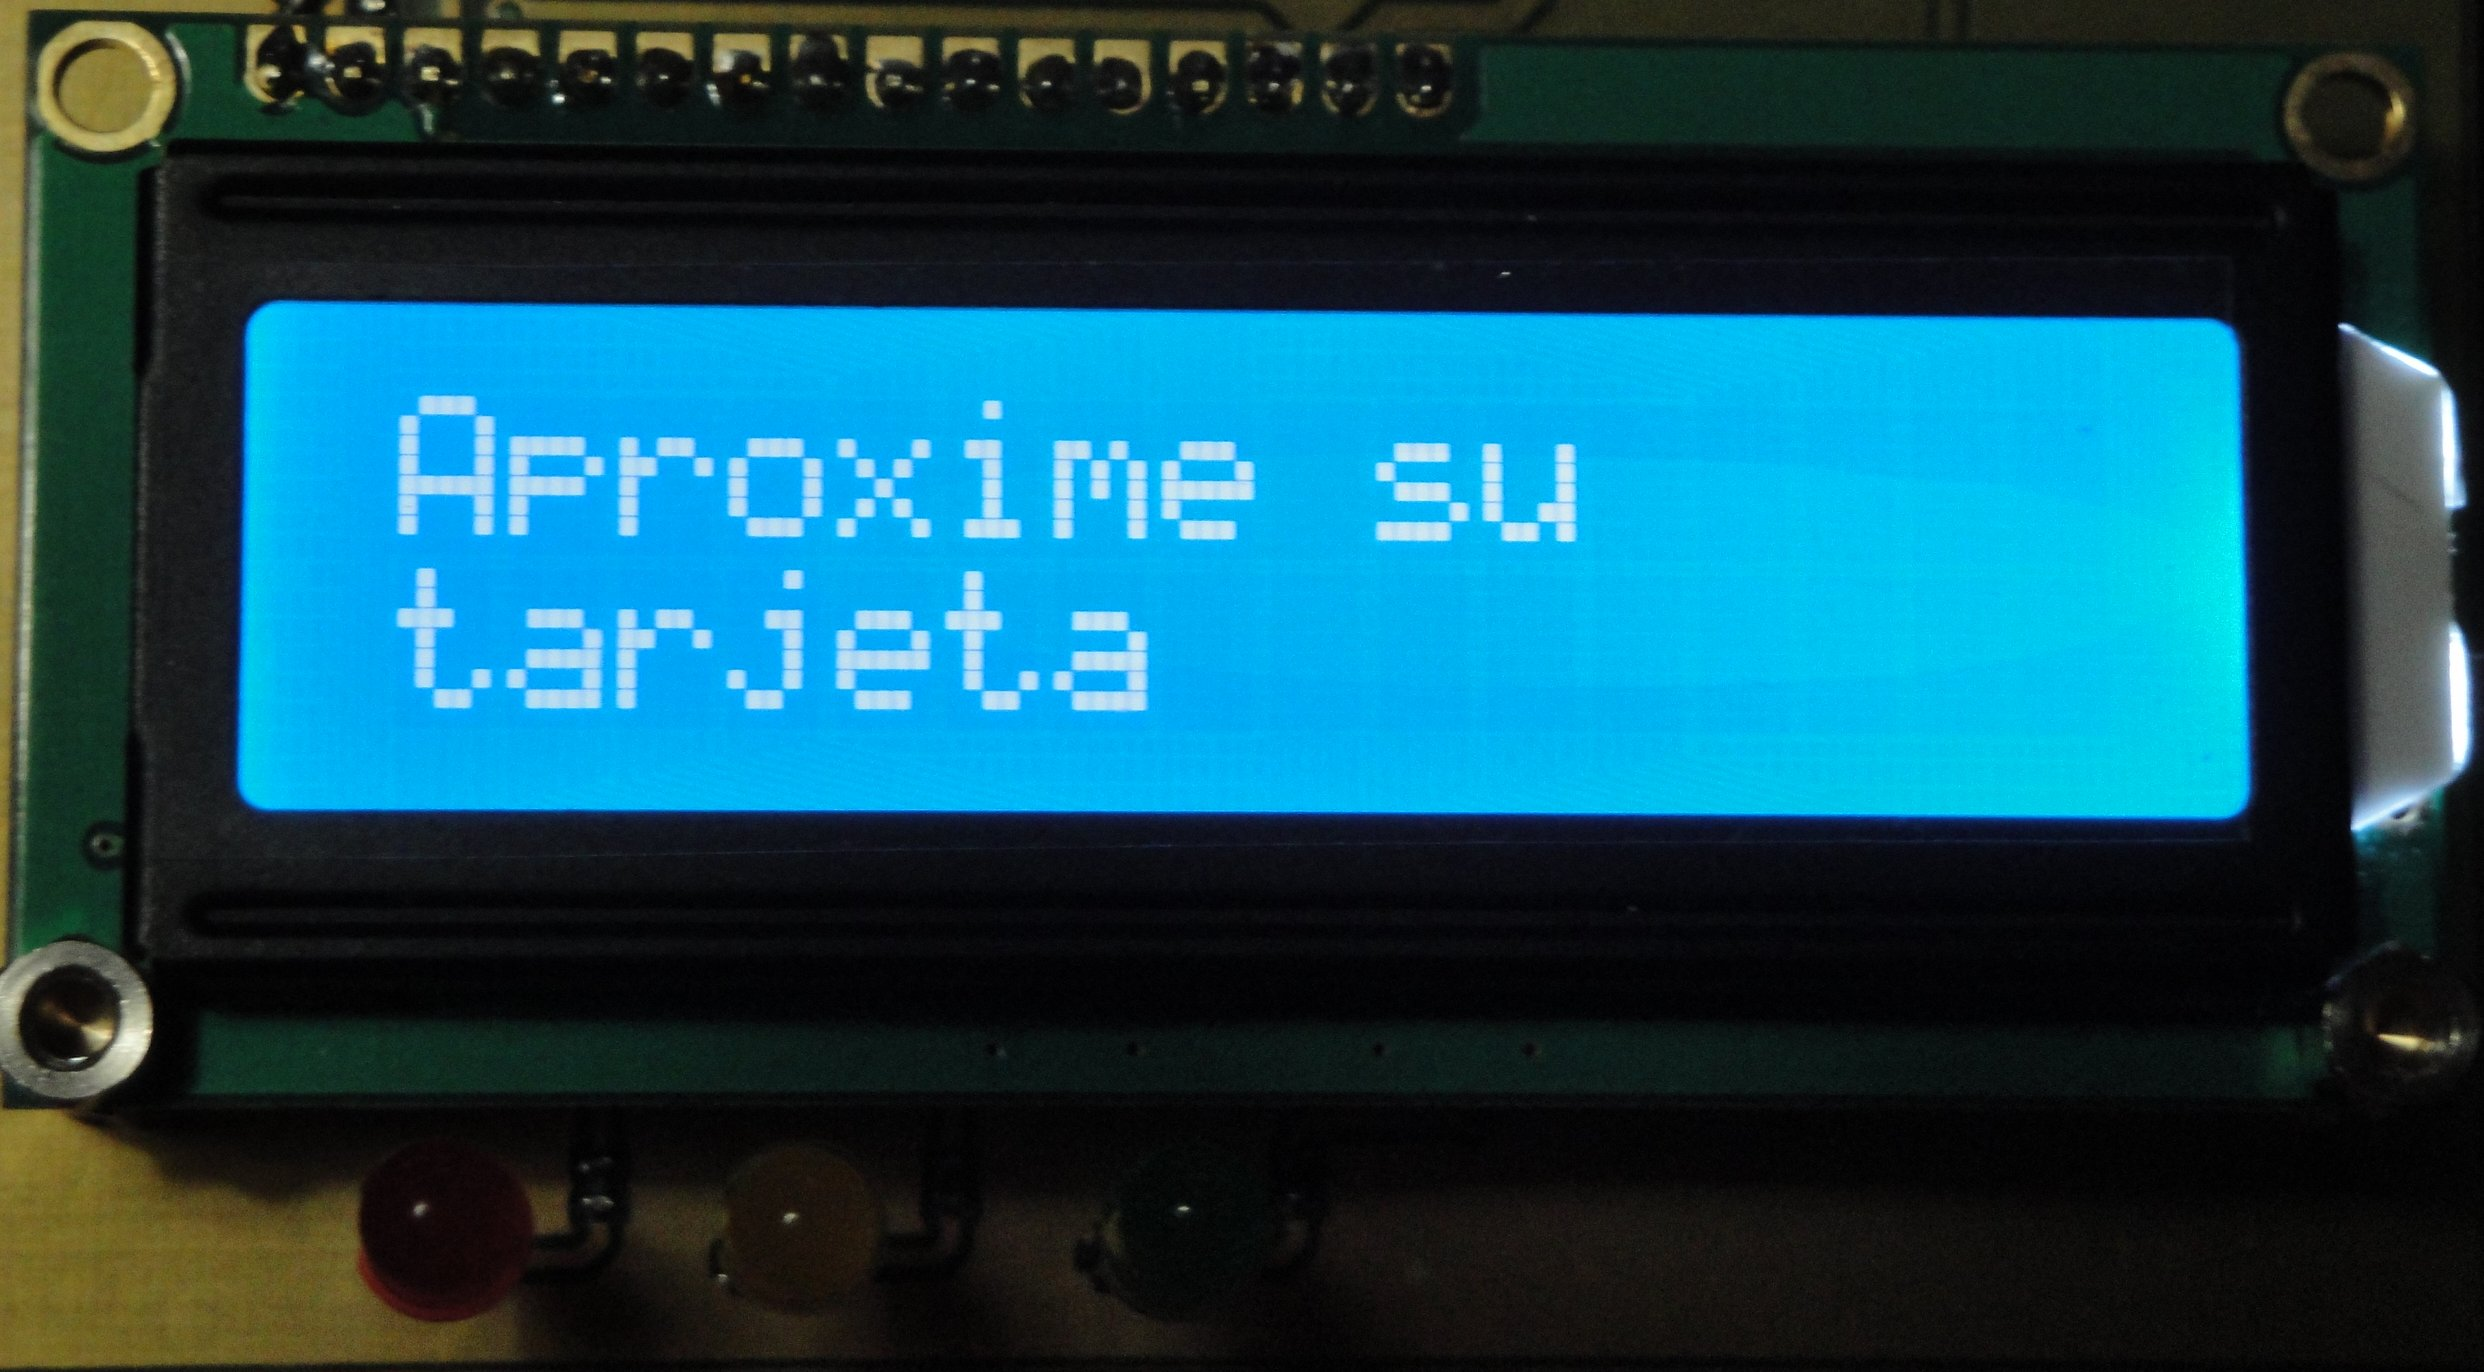
\includegraphics[scale=.08]{Imagenes/Aproxime.jpg}
		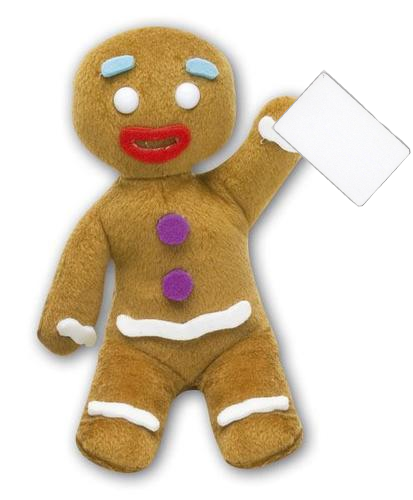
\includegraphics[scale=.35]{Imagenes/pinpon_tarj.png}
	\end{center}
\end{frame}	

\begin{frame}
	\frametitle{Descripción general de funcionamiento}
	\begin{center}
		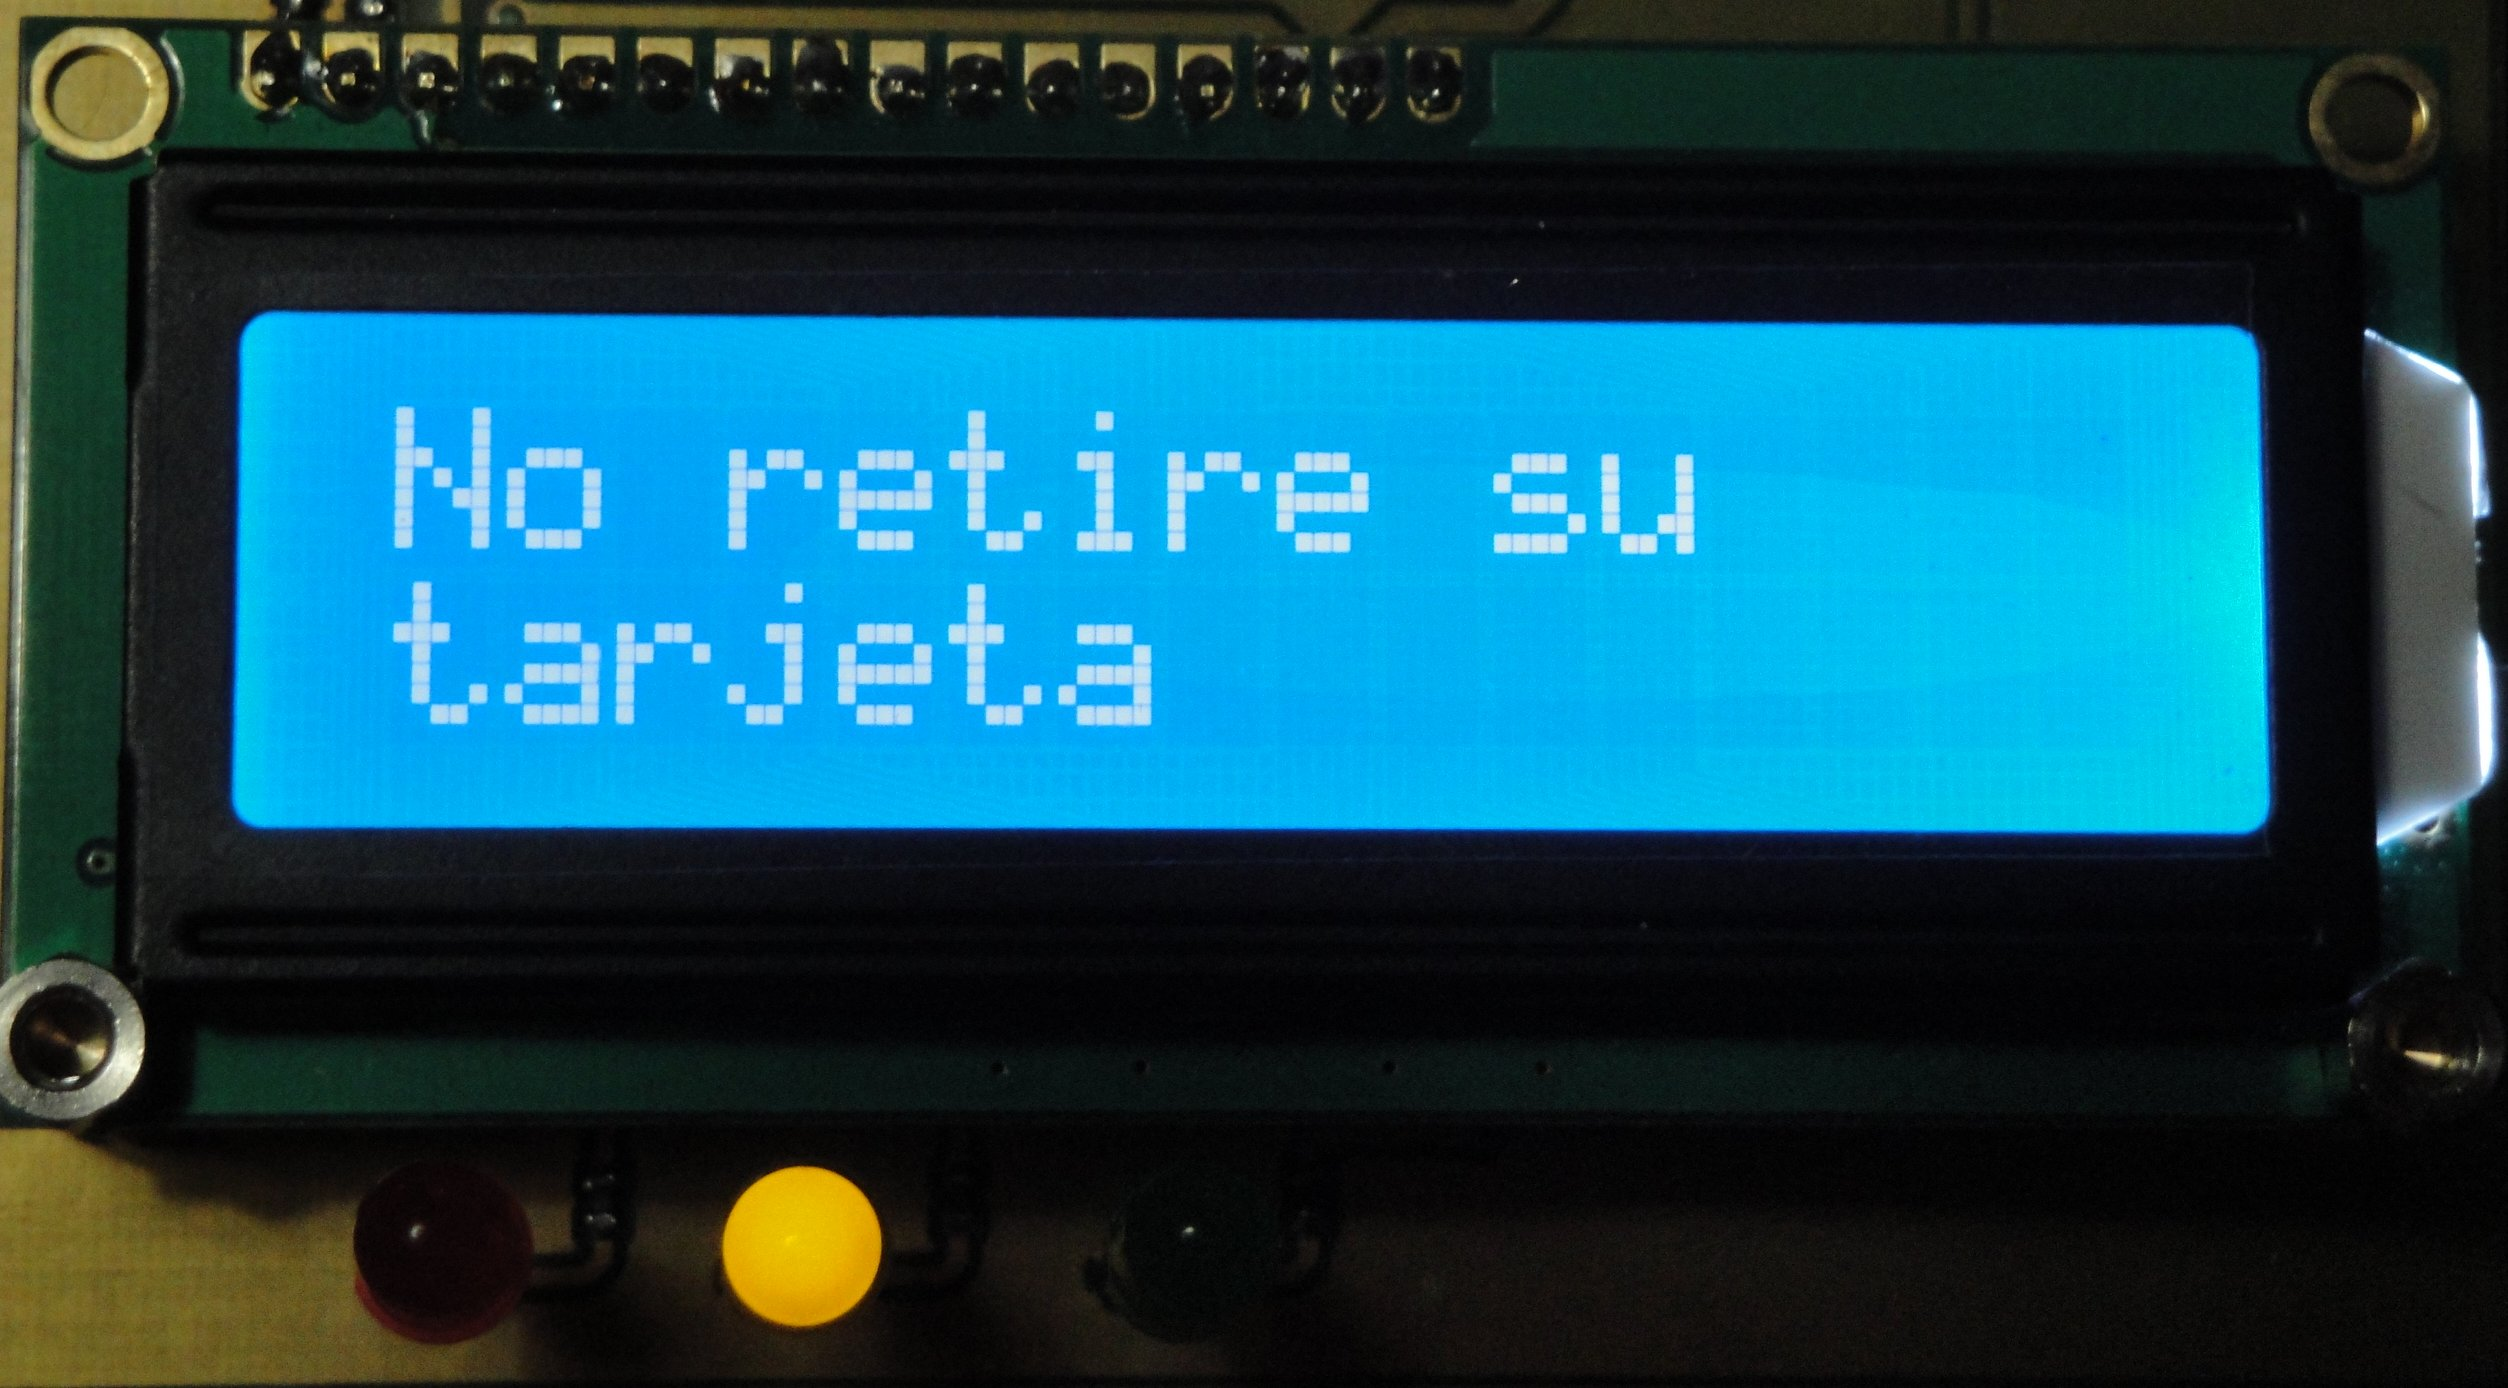
\includegraphics[scale=.08]{Imagenes/noretire.jpg}
		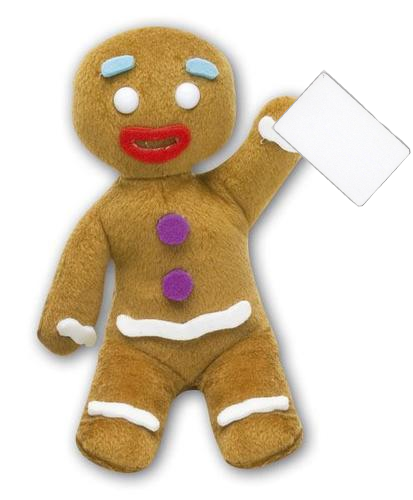
\includegraphics[scale=.35]{Imagenes/pinpon_tarj.png}
	\end{center}
\end{frame}	

\begin{frame}
	\frametitle{Descripción general de funcionamiento}
	\begin{center}
		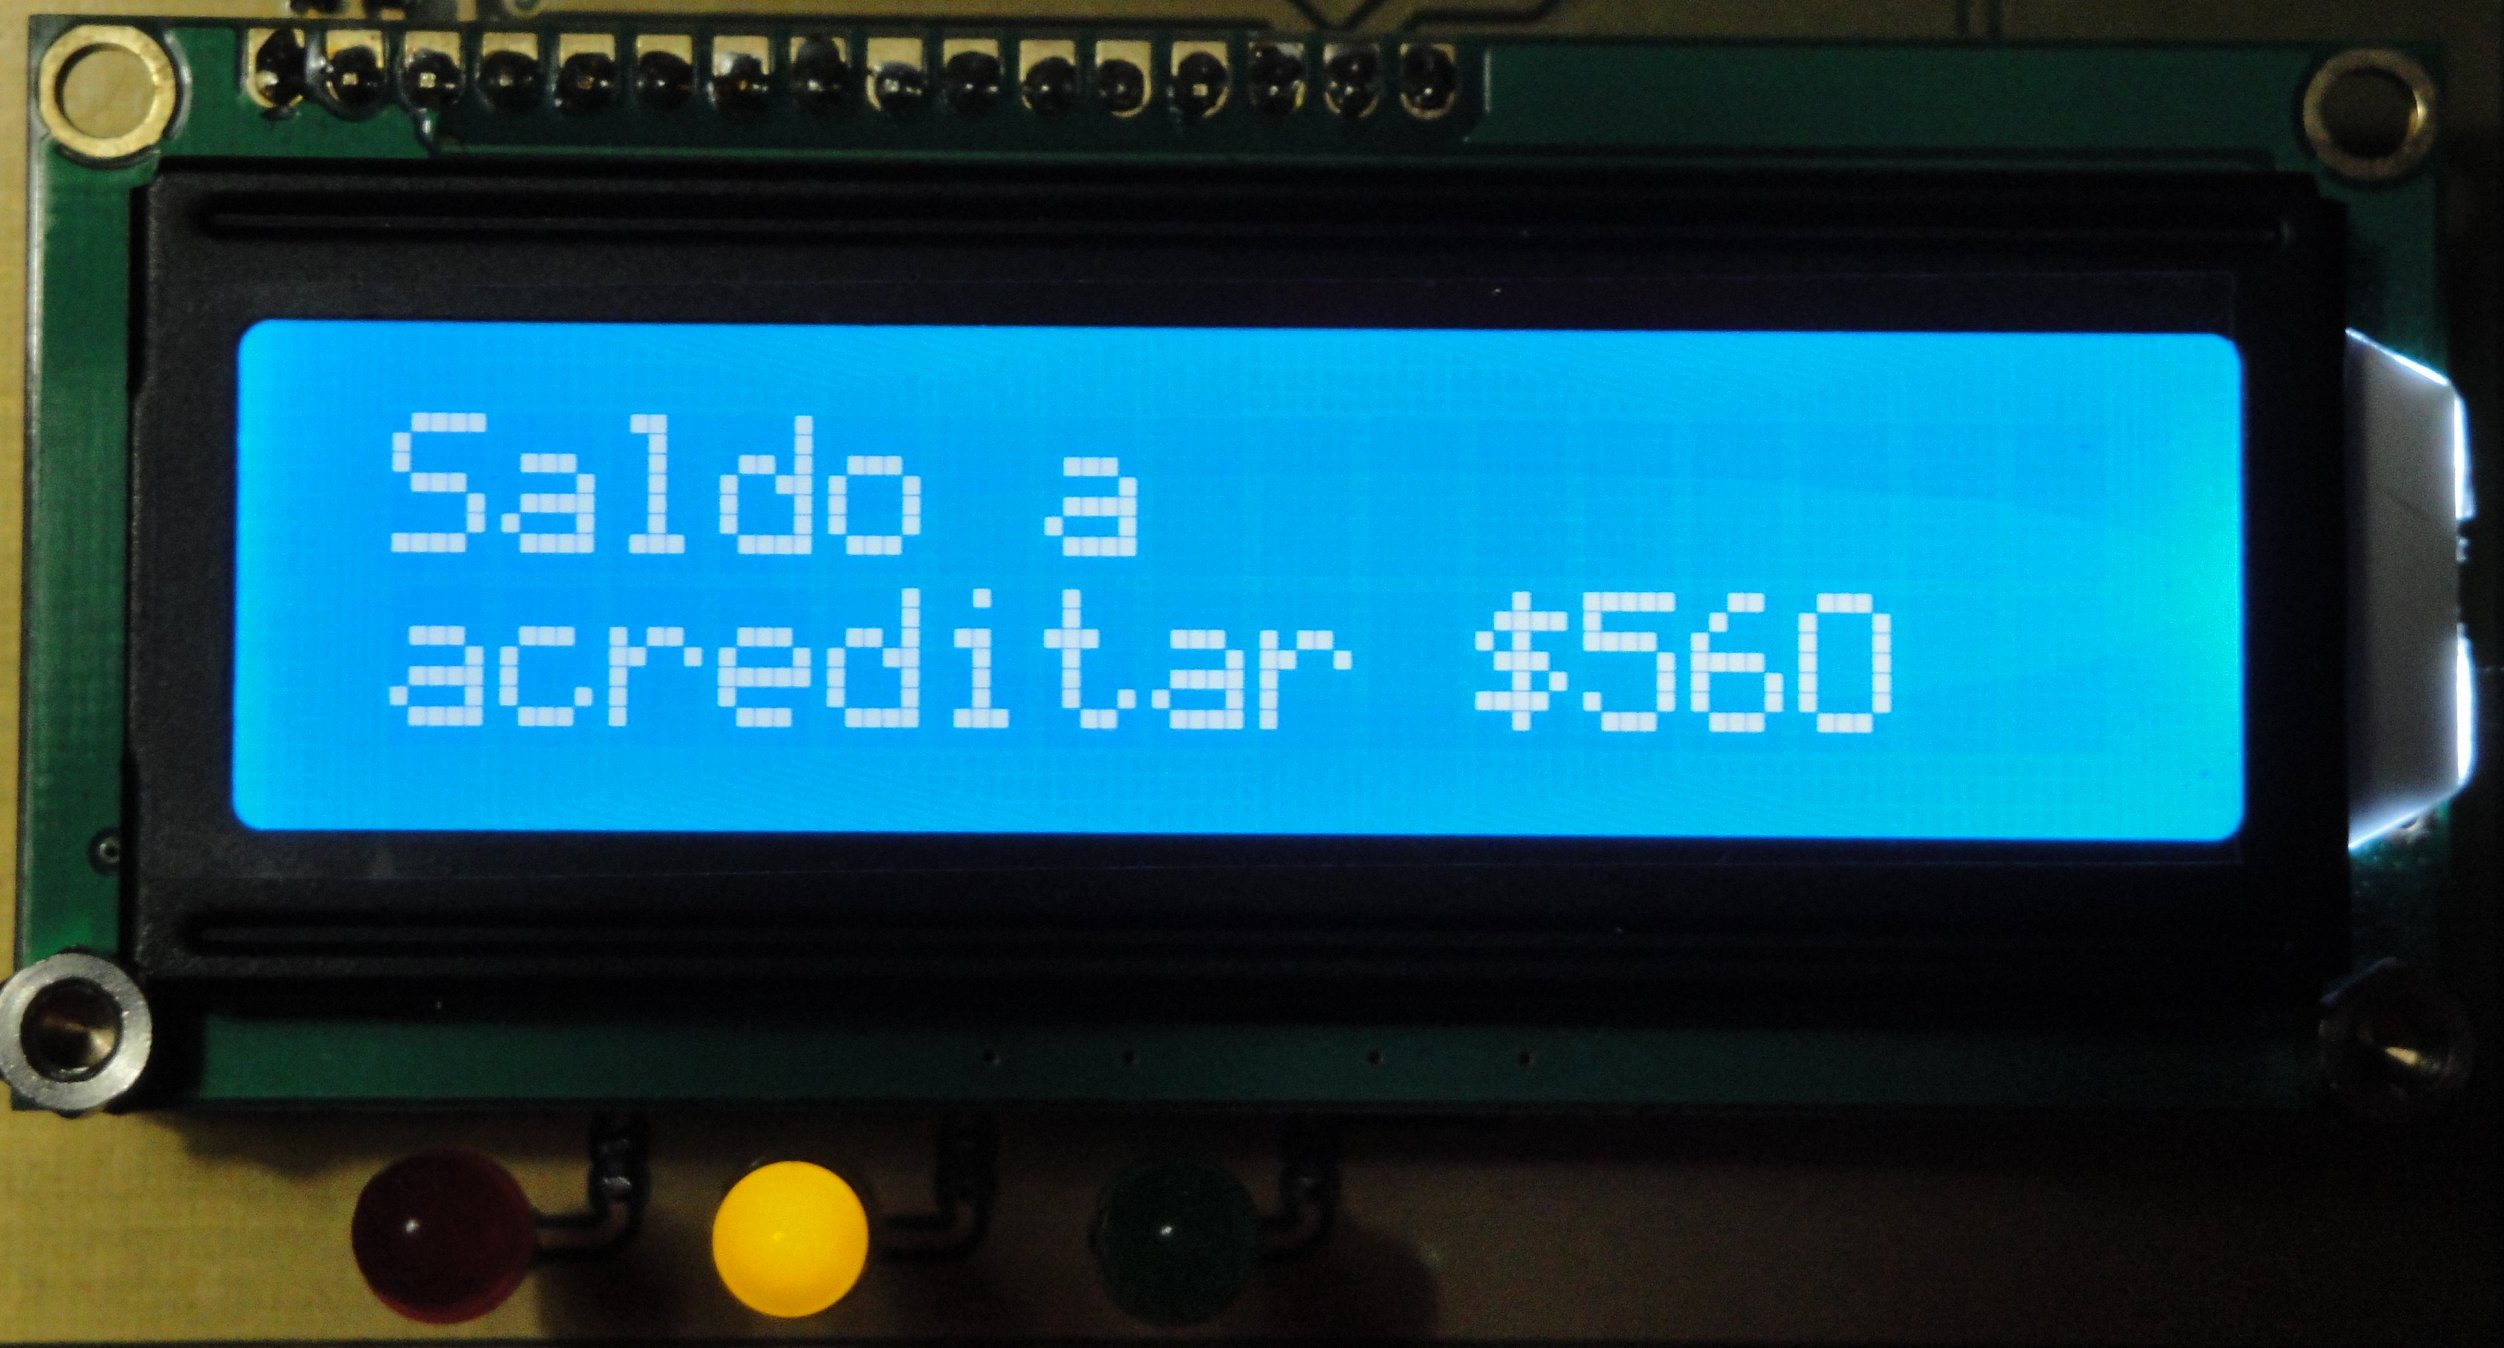
\includegraphics[scale=.08]{Imagenes/saldoacreditar.jpg}
		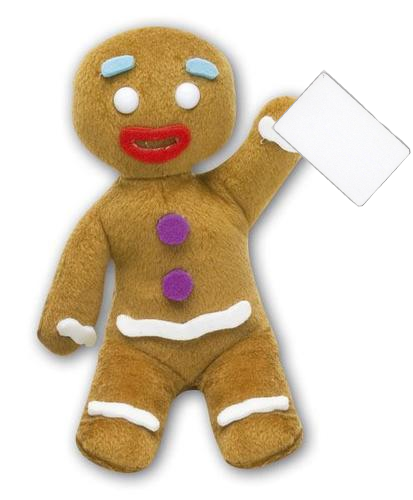
\includegraphics[scale=.35]{Imagenes/pinpon_tarj.png}
	\end{center}
\end{frame}	

\begin{frame}
	\frametitle{Descripción general de funcionamiento}
	\begin{center}
		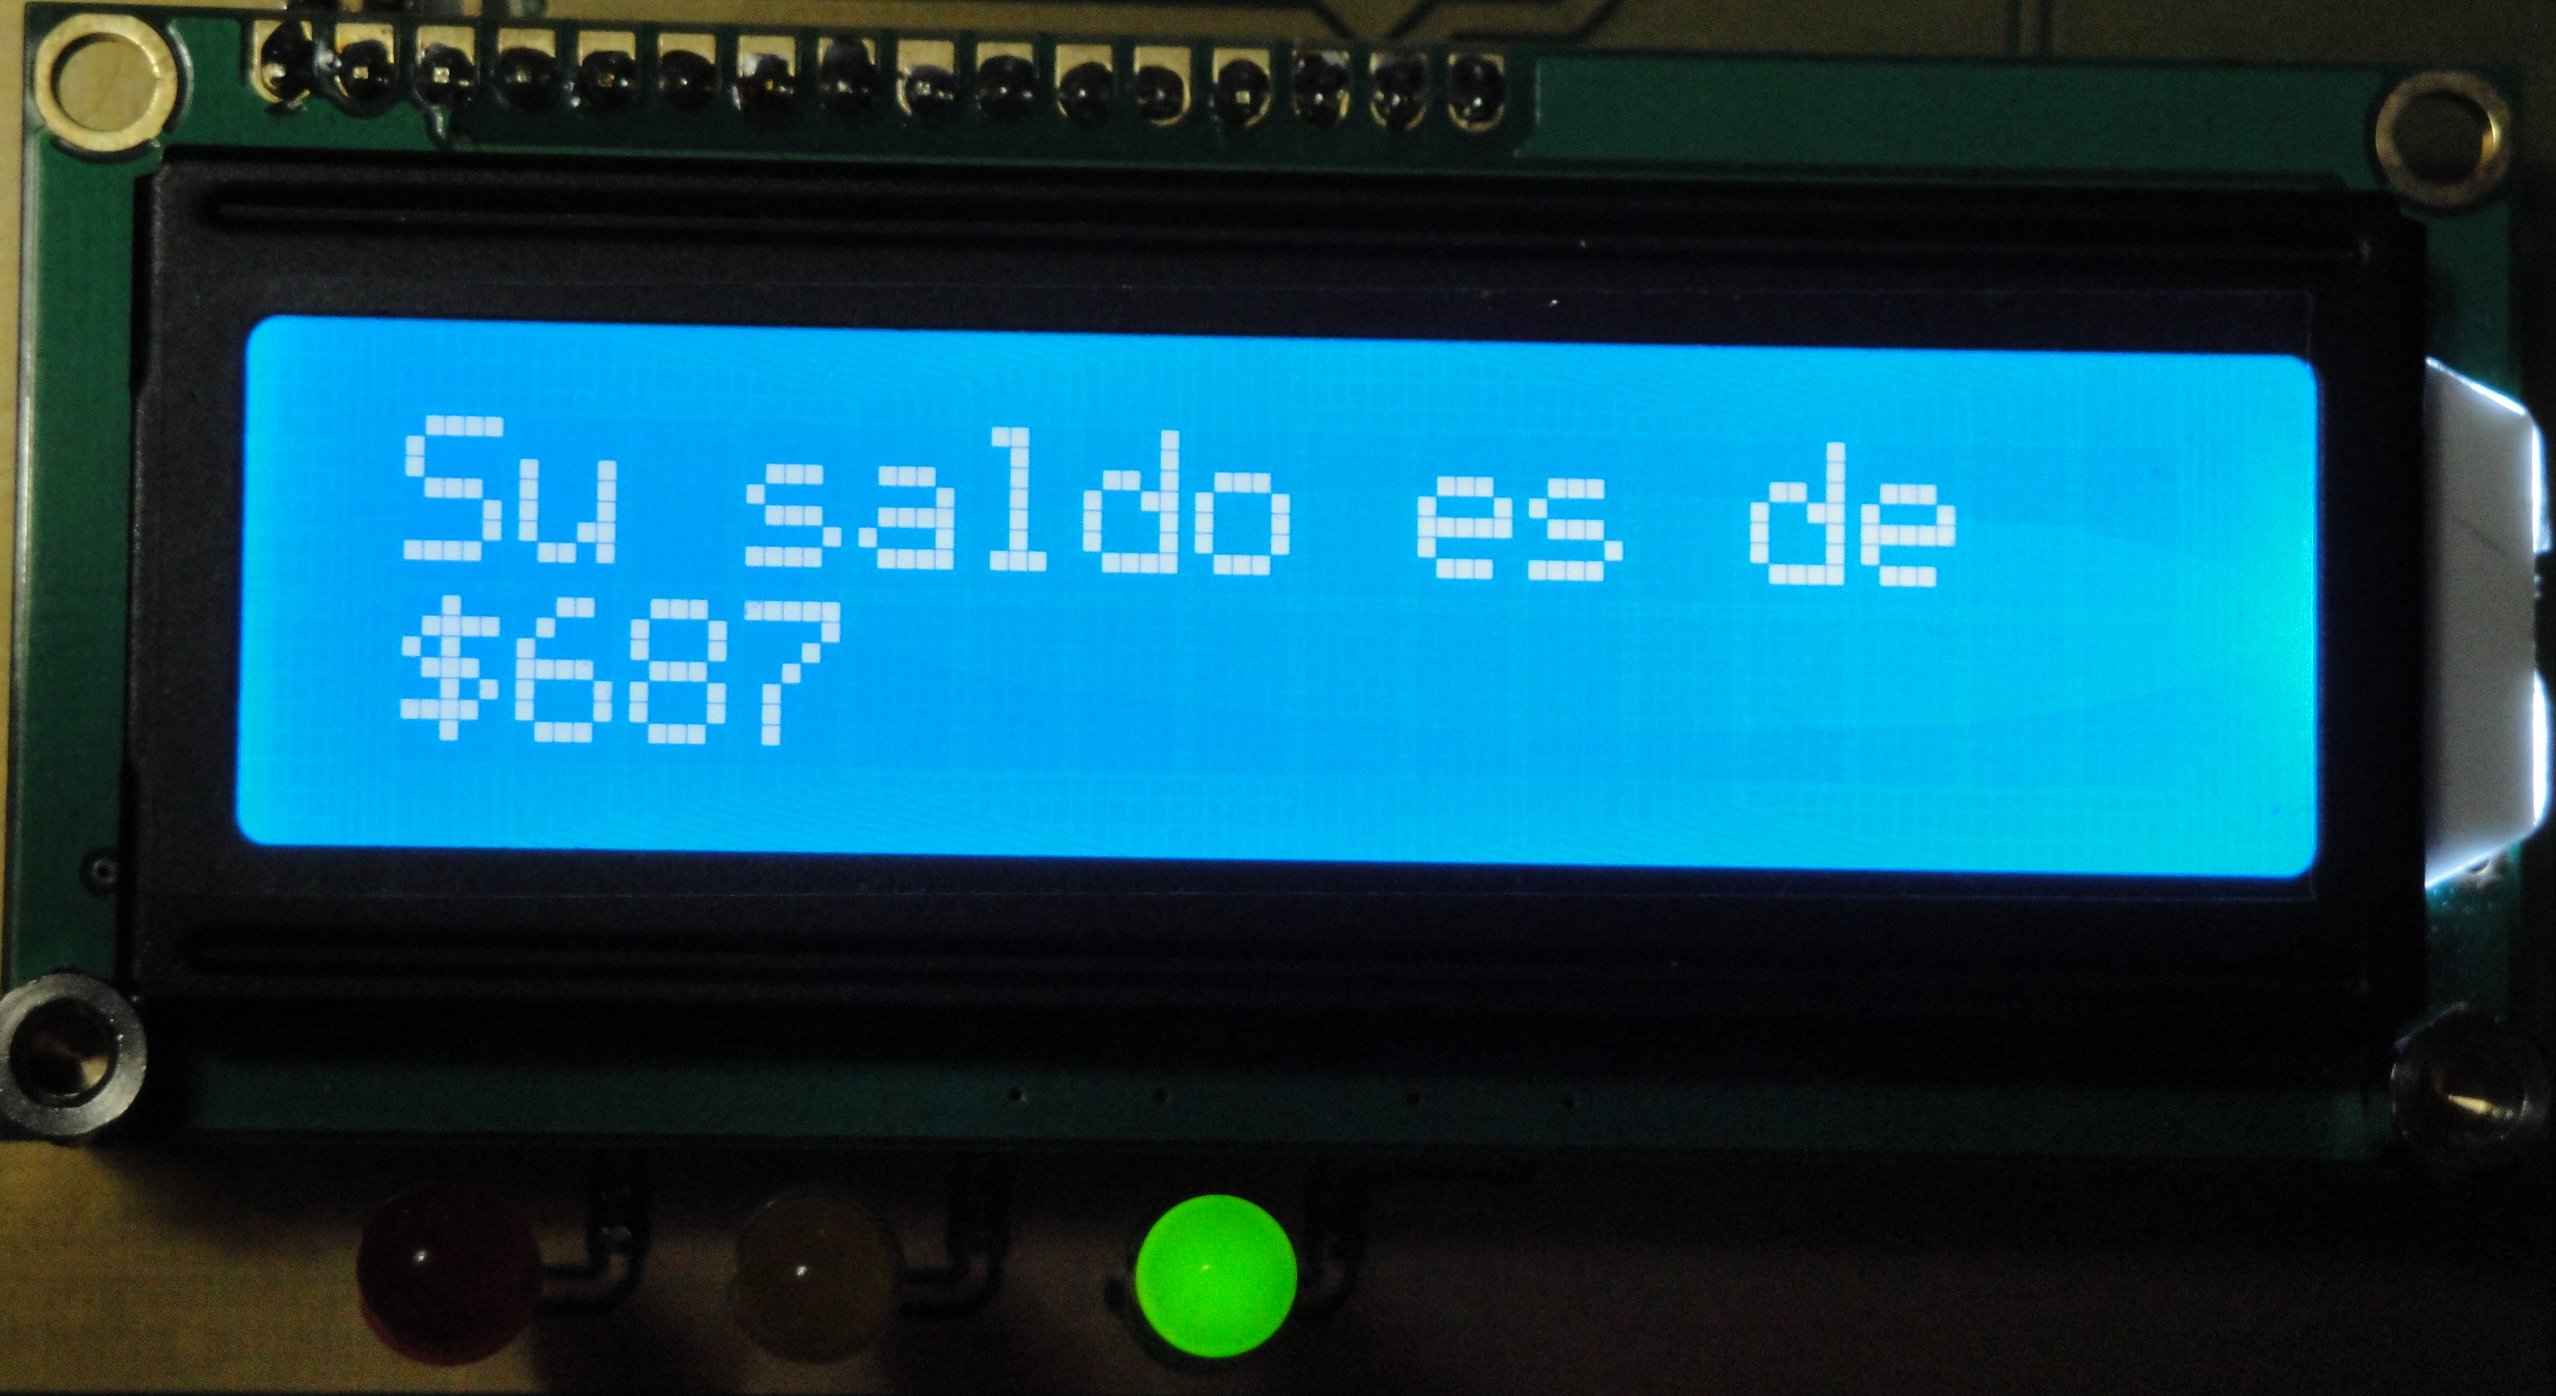
\includegraphics[scale=.08]{Imagenes/saldode.jpg}
		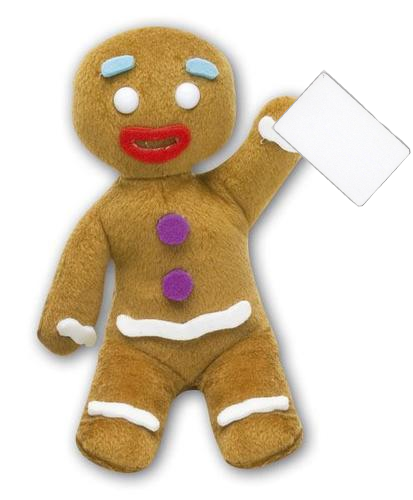
\includegraphics[scale=.35]{Imagenes/pinpon_tarj.png}
	\end{center}
\end{frame}	

\begin{frame}
	\frametitle{Descripción general de funcionamiento}
	\begin{center}
		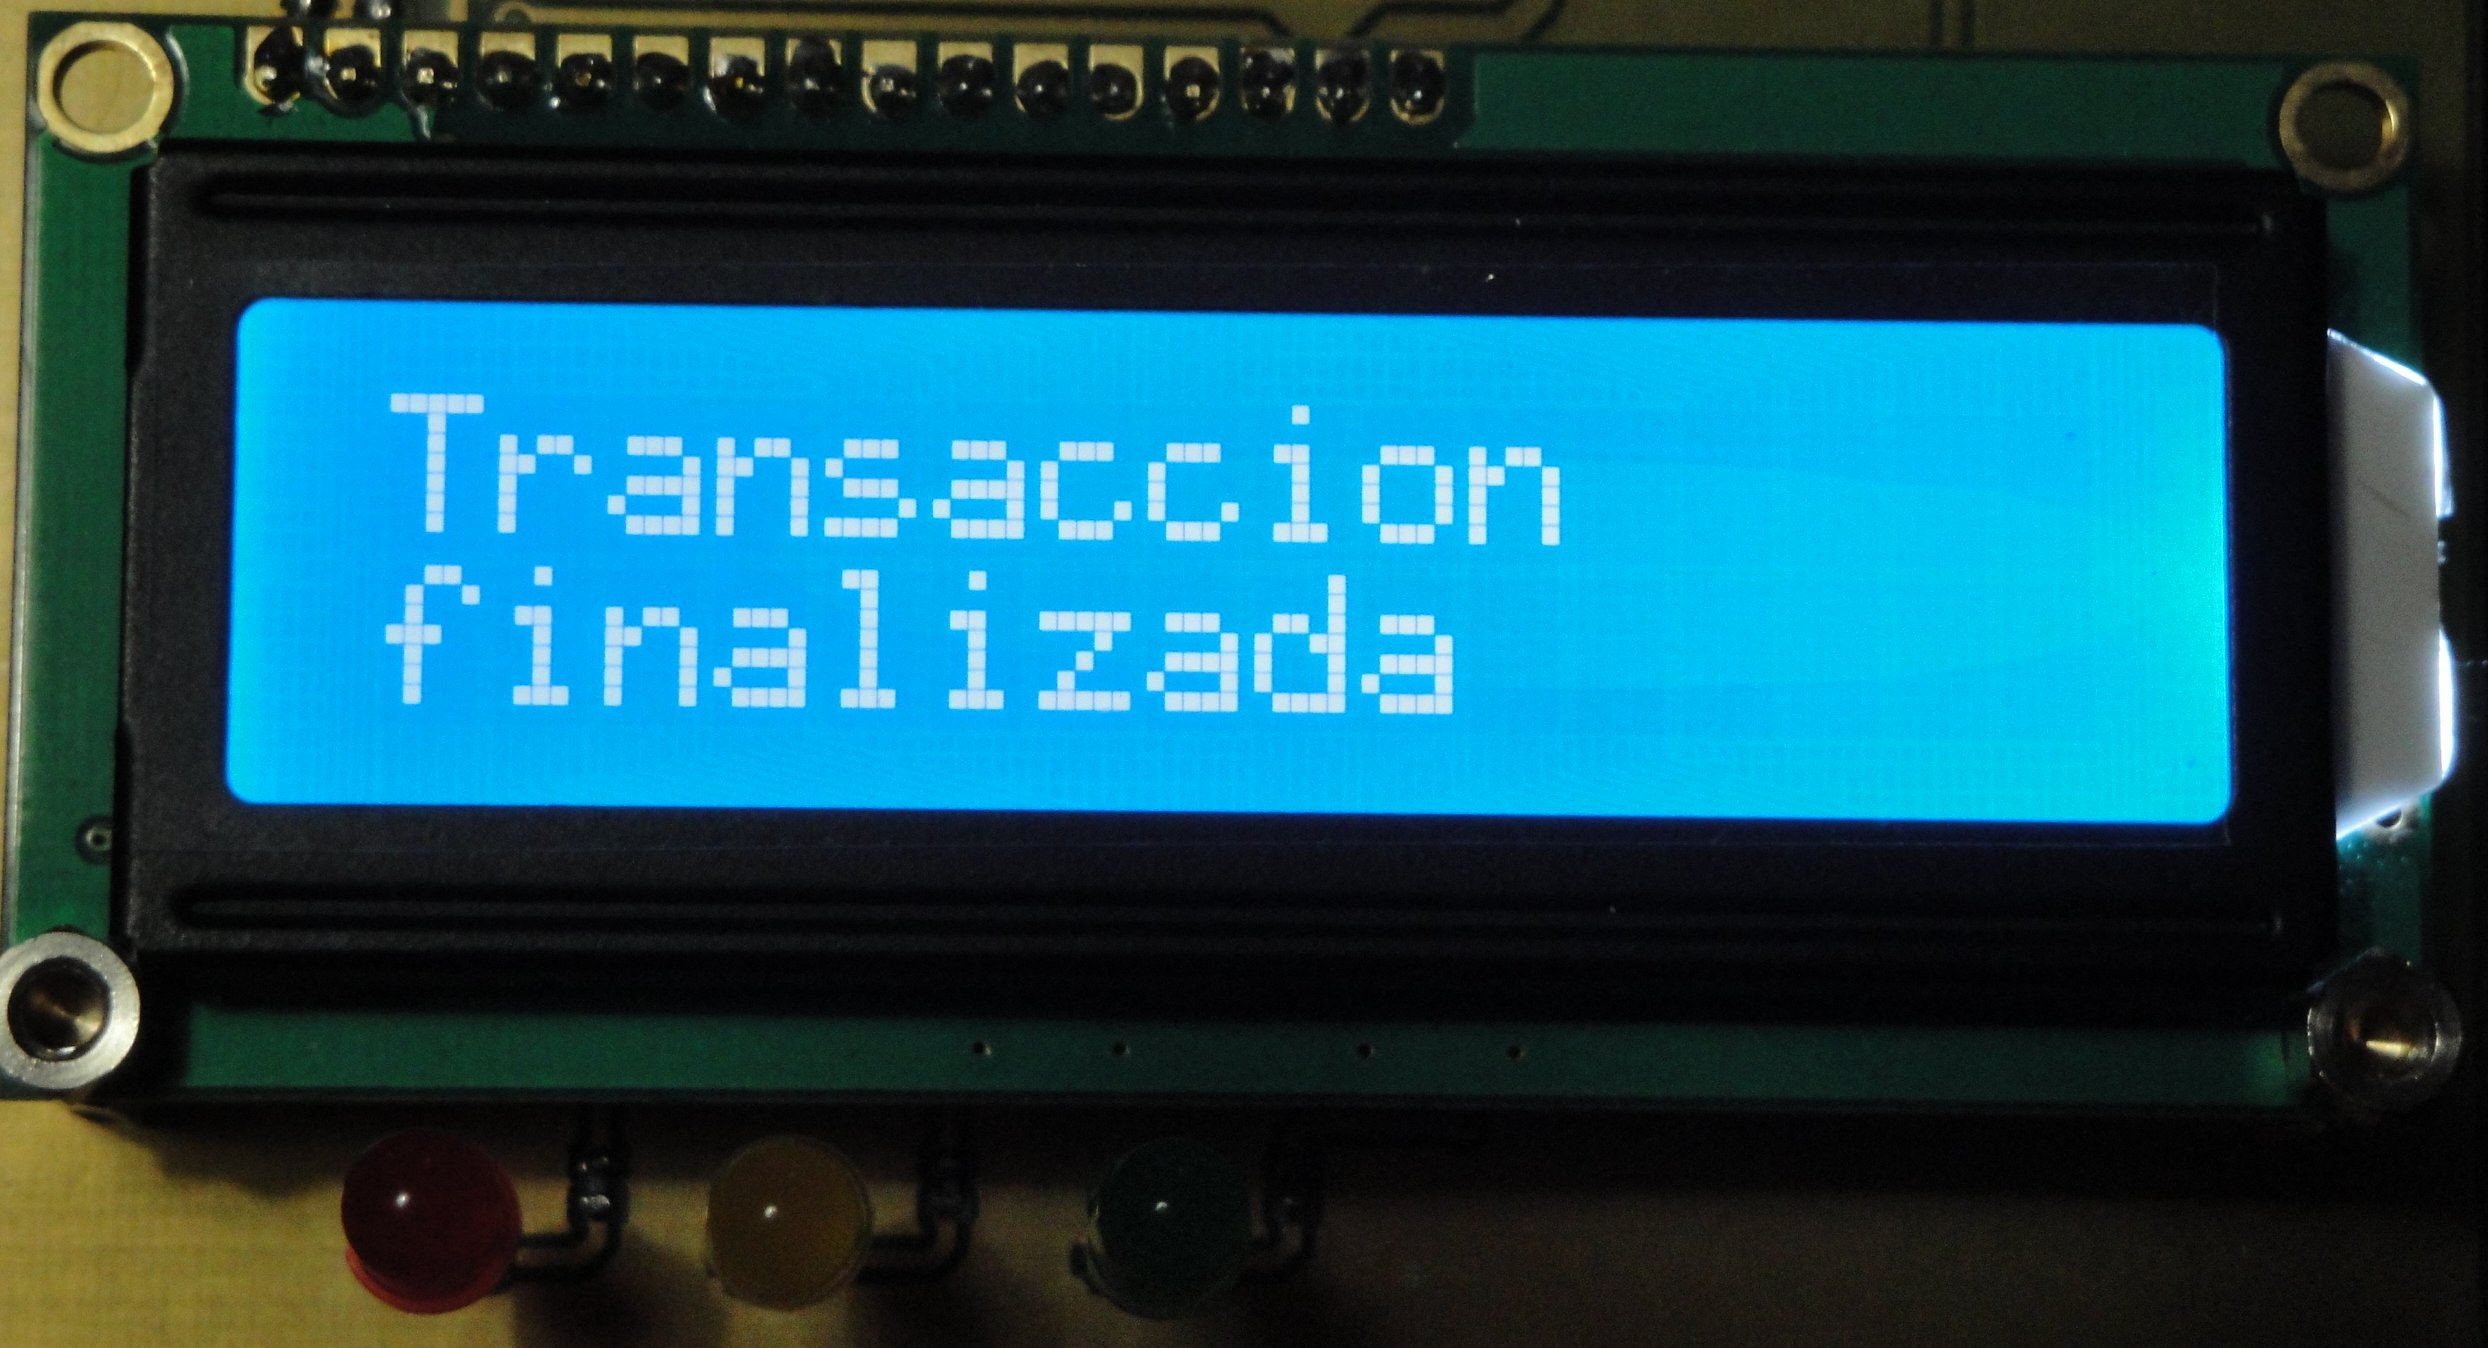
\includegraphics[scale=.08]{Imagenes/fin.jpg}
		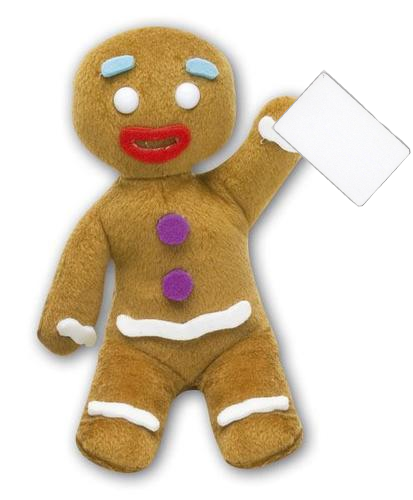
\includegraphics[scale=.35]{Imagenes/pinpon_tarj.png}
	\end{center}
\end{frame}	

\begin{frame}
	\frametitle{Descripción general de funcionamiento}
	\begin{center}
		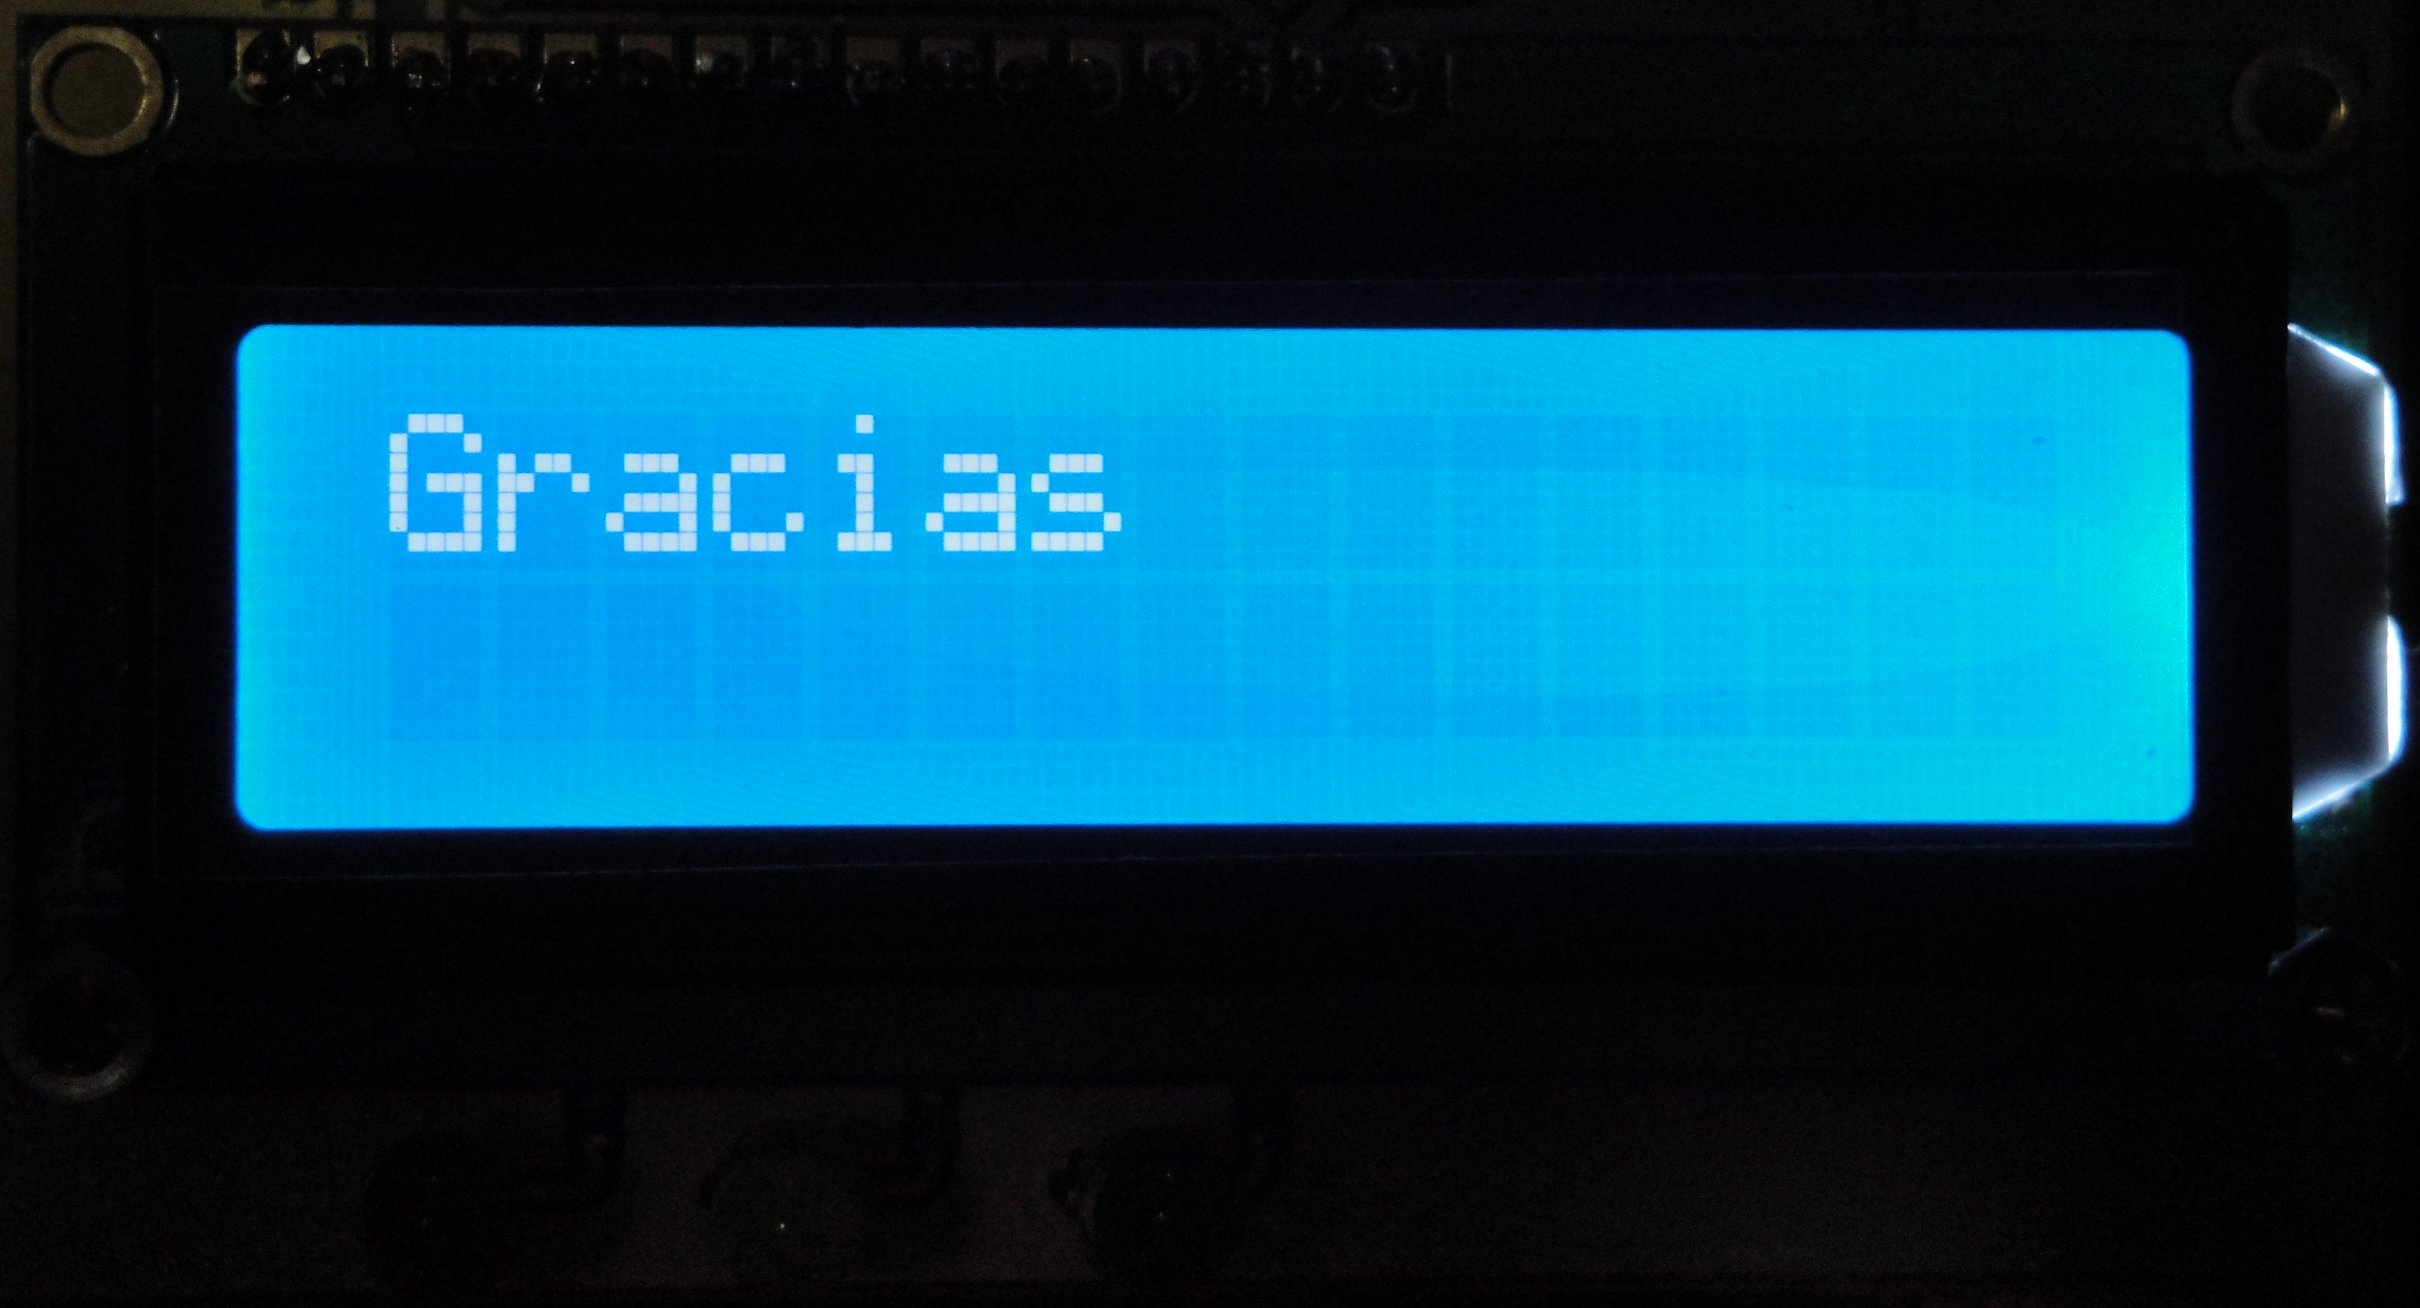
\includegraphics[scale=.08]{Imagenes/grax.jpg}
		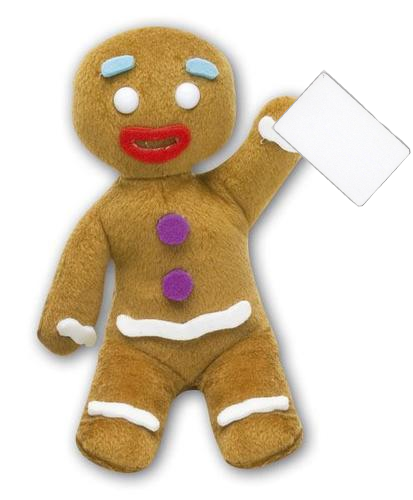
\includegraphics[scale=.35]{Imagenes/pinpon_tarj.png}
	\end{center}
\end{frame}	
%%%%%%%%%%%%%%%%%

\begin{frame}
	\frametitle{Costos}
	\begin{itemize}
		\item \textcolor{gray}{Introducción}
		\item \textcolor{gray}{Objetivos}
		\item \textcolor{gray}{Hardware}
		\item \textcolor{gray}{Software}
		\item \textcolor{gray}{Ensayos}
		\item \textcolor{gray}{Descripción general del funcionamiento}
		\item \textcolor{red}{\bf{Costos}}
		\item \textcolor{gray}{Posibles Mejoras}
		\item \textcolor{gray}{Conclusiones y Logros}
	\end{itemize}
\end{frame}

\begin{frame}
	\frametitle{Costos}
	\begin{block} <2-> {Presupuesto}
		\begin{center}
			Planificado U\$S1500 - Invertido U\$S1400
		\end{center}
	\end{block}

	\bigskip
	\begin{itemize}
		\item <3-> No incluye mano de obra

		\bigskip
		\item <4-> Se incluyen gastos extra (SBC, VLT)

		\bigskip
		\item <5-> Origen de PCBs influyen significativamente
	\end{itemize}
\end{frame}	

\begin{frame}
	\frametitle{Costos}
	\begin{itemize}
		\item[] Costo por unidad:
	\end{itemize}
	
	\begin{table}[htbp]
	\begin{tabular}{|l|r|r|r|}
		\hline
		\multicolumn{1}{|c|}{\textbf{Descripción }} & \multicolumn{1}{c|}{\textbf{Uruguay (U\$S)}} & \multicolumn{1}{c|}{\textbf{China (U\$S)}} \\ \hline
		SBC & 150 & 150 \\ \hline
		Conversor de nivel VLT & 50,56 & 25,16 \\ \hline
		Módulo SCUI & 80,14 & 32,54 \\ \hline
		Lector/escritor RFID & 93,92 & 33,88 \\ \hline
		\multicolumn{1}{|r|}{\textbf{Total}} & 374,62 & 241,58 \\ \hline
	\end{tabular}
	\end{table}
	
	\begin{itemize}
		\item[] Los costos pueden bajar más aún
	\end{itemize}
\end{frame}	

\begin{frame}
	\frametitle{Posibles Mejoras}
	\begin{itemize}
		\item \textcolor{gray}{Introducción}
		\item \textcolor{gray}{Objetivos}
		\item \textcolor{gray}{Hardware}
		\item \textcolor{gray}{Software}
		\item \textcolor{gray}{Ensayos}
		\item \textcolor{gray}{Descripción general del funcionamiento}		
		\item \textcolor{gray}{Costos}
		\item \textcolor{red}{\bf{Posibles Mejoras}}
		\item \textcolor{gray}{Conclusiones y Logros}
	\end{itemize}
\end{frame}

\begin{frame}
	\frametitle{Posibles Mejoras}
	\begin{itemize}
		\item <2-> Terminar de integrar lector/escritor de tarjetas de contacto a PCSC-Lite

		\bigskip		
		\item <3-> Realizar blindaje para la antena RFID
		
		\bigskip		
		\item <4-> Implementar comunicación con un servidor
				
		\bigskip		
		\item <5-> Fabricar carcasa
		
		\bigskip		
		\item <6-> Batería de respaldo
		
		\bigskip		
		\item <7-> Migrar de SD a NAND Flash

		\bigskip		
		\item <8-> Integrar todo a un único PCB
	\end{itemize}
\end{frame}	

\begin{frame}
	\frametitle{Conclusiones y Logros}
	\begin{itemize}
		\item \textcolor{gray}{Introducción}
		\item \textcolor{gray}{Objetivos}
		\item \textcolor{gray}{Hardware}
		\item \textcolor{gray}{Software}
		\item \textcolor{gray}{Ensayos}
		\item \textcolor{gray}{Descripción general del funcionamiento}		
		\item \textcolor{gray}{Costos}
		\item \textcolor{gray}{Posibles Mejoras}
		\item \textcolor{red}{\bf{Conclusiones y Logros}}
	\end{itemize}
\end{frame}

\begin{frame}
	\frametitle{Conclusiones y Logros}
	
	\begin{columns}	
		\begin{column}{9cm}
			\begin{itemize}
				\item <2-> Se logró realizar un prototipo para recarga y/o consulta de tarjetas RFID

				\bigskip		
				\item <3-> Cambio de SBC en el momento adecuado

				\bigskip
				\item <4-> Trabajo en equipo y perseverancia

				\bigskip				
				\item <5-> Uso de bibliotecas abiertas favorece al cliente
			\end{itemize}		
		\end{column}
		
		\begin{column}{2cm}
			\begin{center}
				\includegraphics <2-> [scale=.2]{Imagenes/sinomas.jpg} 

				\bigskip
				\bigskip
				\includegraphics <4-> [scale=.2]{Imagenes/EQUIPO.jpg}
			\end{center}
		\end{column}
	\end{columns}
\end{frame}

\begin{frame}
	\frametitle{Conclusiones y Logros}
	\begin{columns}
		\begin{column}{8cm}
			\begin{itemize}
				\item <2-> Posiblemente, primer lector/escritor RFID 13,56MHz fabricado y diseñado en 								   Uruguay

				\bigskip		
				\item <3-> PCB lector/escritor de tarjetas RFID en 2 capas
				
				\bigskip		
				\item <4-> Sistema 24/7
			\end{itemize}
		\end{column}
		\begin{column}{3cm}
			\begin{center}
				\includegraphics <4-> [scale=.2]{Imagenes/24-7-365.jpg}
			\end{center}
		\end{column}
	\end{columns}
\end{frame}			

\begin{frame}
	\frametitle{Conclusiones y Logros}
	\begin{columns}
		\begin{column}{6cm}
			\begin{itemize}
				\item[] <2-> Prototipo:
		
				\bigskip
				\begin{itemize}
					\item <3-> Escalable

					\bigskip
					\item <3-> Autónomo

					\bigskip		
					\item <3-> Multipropósito
					\begin{itemize}
						\item <4-> Sistema de transporte
						\item <4-> Venta de servicios
						\item <4-> Control de acceso
						\item <4-> Marcas de personal
					\end{itemize}
				\end{itemize}
			\end{itemize}
		\end{column}
	
		\begin{column}{3cm}
		
		\bigskip
			\includegraphics <4-> [scale=.15]{Imagenes/acceso2.jpg}
		
			\bigskip
			\includegraphics <4-> [scale=.2]{Imagenes/pago2.jpg}
			
			\bigskip
		\end{column}
	\end{columns}
\end{frame}

\begin{frame}
	\frametitle{Conclusiones y Logros}
	\begin{columns}	
		\begin{column}{10cm}
			\begin{itemize}
				\item <2-> Generación de conocimiento

				\bigskip
				\item <3-> Solución académica a un problema real

				\bigskip
				\item <4-> Las empresas deberían buscar soluciones tecnológicas a través de la Universidad 						   como referente de conocimiento. 			
			\end{itemize}
		\end{column}
		\begin{column}{2cm}
			\begin{center}
				\includegraphics <4-> [scale=.3]{Imagenes/udelar.jpg}
			\end{center}
		\end{column}
	\end{columns}
\end{frame}

\begin{frame}
	\frametitle{Gracias Totales}
	\begin{center}		
		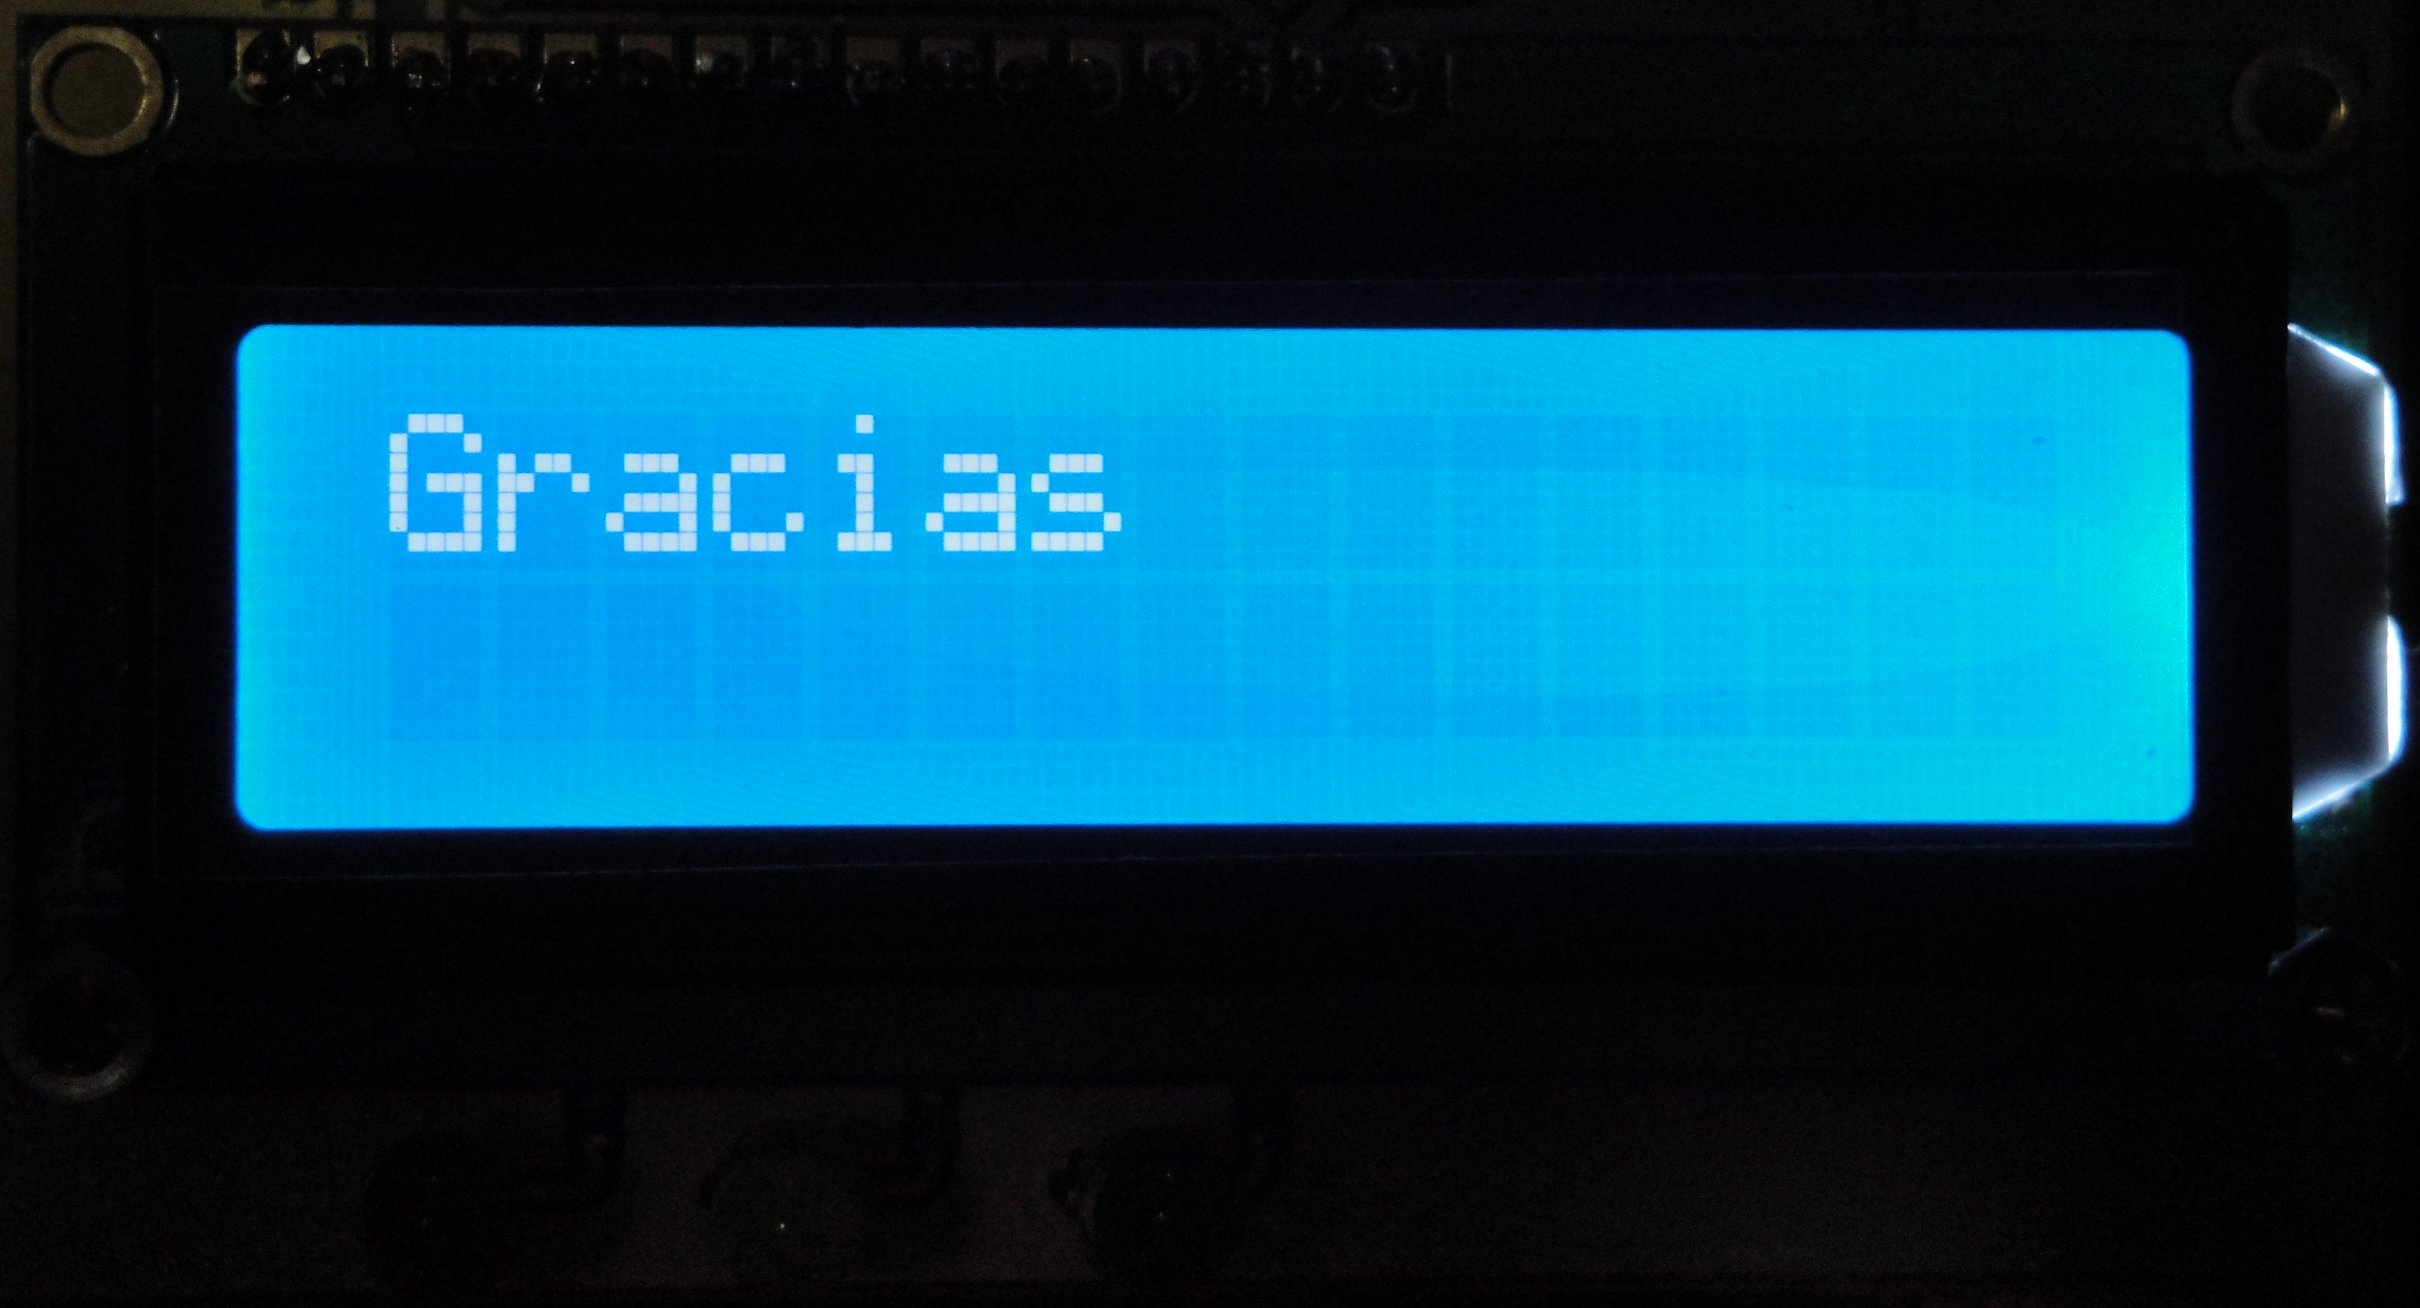
\includegraphics[scale=.1]{Imagenes/grax.jpg}
	\end{center}
\end{frame}

\begin{frame}
	\frametitle{Preguntas}
	\begin{center}
		\bigskip		
		
\includegraphics[scale=.25]{Imagenes/preguntas.jpg}
	\end{center}
\end{frame}

\end{document} 